\documentclass[a4paper, twoside]{article}

%%%%%%%%%%%%%%%%%%%%%%%%%%%%%%%%%%%%%%%%%%%%%%
% Gestion du Français et des accents %
\usepackage[utf8x]{inputenc}
\usepackage[T1]{fontenc}
\usepackage[greek, french]{babel}
%%%%%%%%%%%%%%%%%%%%%%%%%%%%%%%%%%%%%%%%%%%%%%

%\usepackage[UTF8]{ctex}

%%%%%%%%%%%%%%%%%%%%%%%%%%%%%%%%%%%%%%%%%%%%%%
% Gestion des Sections et de la Table des matières %
\setcounter{secnumdepth}{3}
\setcounter{tocdepth}{3}

\usepackage[]{titletoc}
%\titlecontents
%		{section}
%		[left]
%		{au-dessus}
%		{avant (si label)}
%		{avant (sans label)}
%		{remplissage et n°page}
%		[après]



%%%   Section   %%%

\titlecontents
	{section}
	[25pt]
	{\addvspace{0.75pc}}
	{\normalfont\scshape\contentslabel{25pt}}
	{}
	{\normalsize\hfill\bfseries ~\thecontentspage\vspace{-3pt}\hrule}
	[\addvspace{0.5pc}]
	


%%%   Sous-Section   %%%

\titlecontents
	{subsection}
	[75pt]
	{\addvspace{-0.5pc}}
	{\normalfont\small\contentslabel{30pt}}
	{}
	{\normalsize\dotfill\small\thecontentspage}
	[]



%%%   Sous-sous-Section   %%%

\titlecontents
	{subsubsection}
	[125pt]
	{\addvspace{-0.5pc}}
	{\normalfont\footnotesize\contentslabel{30pt}\itshape}
	{}
	{\normalsize\hfill\footnotesize\itshape\thecontentspage}
	[]
	
\contentsfinish
%%%%%%%%%%%%%%%%%%%%%%%%%%%%%%%%%%%%%%%%%%%%%%

%%%%%%%%%%%%%%%%%%%%%%%%%%%%%%%%%%%%%%%%%%%%%%
% Gestion des marges du document %

\usepackage{geometry}

\geometry{
paperwidth=21cm,
%width=15.5cm,
left=3cm,
right=3cm,
paperheight=29.7cm,
%height=26.5cm,
top=3cm,
bottom=3cm,
headheight=0cm,
headsep=0cm,
footskip=1cm
}
%%%%%%%%%%%%%%%%%%%%%%%%%%%%%%%%%%%%%%%%%%%%%%

%%%%%%%%%%%%%%%%%%%%%%%%%%%%%%%%%%%%%%%%%%%%%%
% Gestion des numéros de page et des titres de section %

\usepackage{fancyhdr}

\pagestyle{fancy}
\fancyhf{} % Efface tous les en-têtes et pieds de page
\fancyfoot[RO]{\thepage}
\fancyfoot[LE]{\thepage}
\renewcommand{\headrulewidth}{0pt}
\pagestyle{fancy}

%%%%%%%%%%%%%%%%%%%%%%%%%%%%%%%%%%%%%%%%%%%%%%

\usepackage{graphicx}
\usepackage{setspace}
\usepackage{mathtools}
\usepackage{rotating}
\usepackage{multirow}

%\usepackage[mathletters]{ucs}

\DeclareFontEncoding{LS1}{}{}
\DeclareFontSubstitution{LS1}{stix}{m}{n}
\DeclareSymbolFont{symbols4}{LS1}{stixbb}{m}{it}
\DeclareMathSymbol{\varhexagonblack}{\mathord}{symbols4}{"DD}
\DeclareMathSymbol{\hexagonblack}   {\mathord}{symbols4}{"DE}


\usepackage{setspace}
\usepackage{amssymb}
\usepackage{numprint}

\def\nbR{\ensuremath{\mathrm{I\! R}}}


\renewcommand{\thesection}{\Roman{section}}
\renewcommand{\thesubsubsection}{\roman{subsubsection}}

\usepackage{xlop}
\usepackage{ulem}

\parindent=1cm

\usepackage[bottom]{footmisc}
\usepackage[dvipsnames]{xcolor}

\begin{document}

\begin{titlepage}
	\begin{center}

		\Huge	 \textbf{Recueil mathématique}\\
		\bigskip \smallskip

		\Large	 \textbf{$\varhexagonblack$ Section 2 - Géométrie $\varhexagonblack$}\\
		\bigskip

		\large	 Clément \sc{Campana}  \\
		\smallskip

		\normalfont	Juillet 2022 \\

	\end{center}

	%\onehalfspacing
	\doublespacing
	\tableofcontents
	\singlespacing

\end{titlepage}





% -------------------------------------------------------------

\section{Introduction à la Géométrie}

La géométrie est une branche des mathématiques étudiant les objets constructibles sur un plan ou dans l'espace.
Pour cela, on y manipule divers outils, comme les points, les lignes ou les angles.
Ils nous permettent de créer des objets plus complexes, comme les cercles ou les polygones.

\medbreak

Dans les prochaines pages, nous travaillerons uniquement dans le plan, c'est-à-dire sur des figures planes,
pouvant se tracer sur une feuille de papier. Ainsi, nous ferons de la \textbf{géométrie euclidienne}.
Cependant, il est aussi possible de faire de la géométrie dans l'espace
(où l'on peut étudier le cube et la boule par exemple) ou sur des surfaces n'étant pas plates
(on parle alors de géométrie non euclidienne\footnote{La géométrie euclidienne
	repose sur des faits considérés comme admis, sans être démontrés (ce sont des Axiomes).
	Et il est possible, en modifiant un, de totalement changer la courbure de la géométrie
	dans laquelle nous nous trouvons, pour en savoir plus rendez-vous en Annexe (page n°\pageref{geo_non_euclidienne}) }).

\subsection{Points}

Les points sont les briques élémentaires à partir desquels il est possible de construire toutes les autres figures géométriques.
Un point n'a pas de dimension (pas de longueur, ni de largeur et encore moins de hauteur).
On peut ainsi le considérer comme étant \textbf{infiniment petit}.

Mais évidemment, comme il est impossible de voir ou de tracer un objet de cette nature,
il est nécessairement représenté avec une certaine taille. Néanmoins il ne faut pas oublier cette définition théorique du point,
car en géométrie, ce que l'on trace n'est que le reflet imparfait des objets sur lesquels on raisonne.

\medbreak

Pour distinguer un point d'un autre, on les nomme en utilisant les lettres de l'alphabet,
auxquelles on peut ajouter en indice ou d'autres éléments,
afin d'être plus libre dans le choix de la dénomination.

\newpage

\subsection{Segments et Droites}

\subsubsection*{Définitions}

Un \emph{segment} est une ligne finie, comprise entre deux points.
On note le segment allant du point $A$ au point $B$, le segment $[AB]$.

\medbreak

Une \emph{droite} est une ligne infinie, passant par deux points.
On note la droite passant par le point $C$ et le point $D$, la droite $(CD)$.

\medbreak

Il est aussi possible de construire une \emph{demi-droite}, partant d'un point et passant par un autre.
On note la demi-droite partant du point $E$ et passant par le point $F$, la demi-droite $[EF)$.
				Il est aussi possible de construire une demi-droite passant par un point $G$ et s'arrêtant à un point $H$,
				on la notera $(GH]$.

\subsubsection*{Propriétés}

Deux droites sont \emph{parallèles} entre elles si et seulement si, ces droites ne se coupent jamais.
On dira, par exemple, que la droite $(CD)$ est parallèle à la droite $(IJ)$, ou plus synthétiquement $(CD)//(IJ)$.
Deux lignes (segments, droites et demi-droites) sont parallèles si et seulement si,
les droites passant par les points définissant les lignes sont parallèles.
\textit{On gardera la même dénomination, il est possible de dire que le segment $[AB]$ est parallèle à
la demi-droite $[EF)$, et de l'écrire $[AB] // [EF)$.}

\medbreak

Deux lignes sont \emph{perpendiculaires} entre elles si et seulement si, ces deux lignes se coupent
en formant un angle droit (dont la définition est donnée à la page suivante).
On dira que, par exemple, le segment $[AB]$ est perpendiculaire à la droite $(CD)$,
ou de manière plus synthétique à l'écrit $[AB] \bot (CD)$.

\medbreak

Une \emph{médiatrice} est une droite perpendiculaire à un segment passant par son milieu.

Pour savoir comment tracer une médiatrice, rendez-vous page n°\pageref{tracer_mediatrice_bissectrice}.

\medbreak

Deux lignes sont dites \emph{sécantes} si elles se coupent,
si elles se croisent une seule fois, alors elles sont \emph{concourantes}.
Ce point d'intersection est appelé \emph{point de concours}.

\subsubsection*{Notation alternative}

Il est possible de noter une ligne par une lettre minuscule (les majuscules étant
généralement réservées aux points), il est par exemple assez classique de nommer une
droite $d$ ou $d'$ (prononcé \textit{dé prime}).


\subsubsection*{Exemple}

Voici les segments $[AB]$ et $[CD]$, les droites $(EF)$ et la demi-droite $[GH)$ :

\begin{center}
	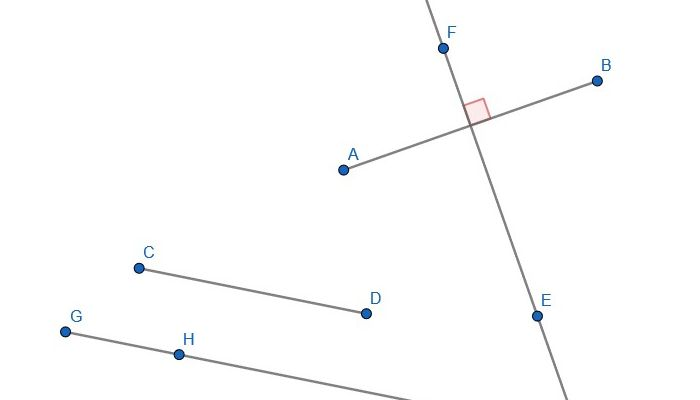
\includegraphics[width=10cm]{Image/Exemple segment droite.jpg}
\end{center}

On remarque que le segment $[CD]$ et la demi-droite $[GH)$ sont parallèles entre eux.
De plus, la droite $(EF)$ est perpendiculaire à $[AB]$, et comme $(EF)$ passe par le milieu de $[AB]$,
$(EF)$ est la médiatrice de $[AB]$.

\newpage

\subsection{Angles}

\subsubsection*{Définition}

Lorsque deux lignes se croisent, elles forment un certain \emph{angle} entre elles au niveau de leur point d'intersection.

\paragraph*{Représentation}
On représente un angle avec un arc de cercle, commençant et se terminant sur les lignes le définissant.
Cette règle s'applique à tous les angles, sauf pour l'\emph{angle droit}
que l'on représente avec une portion de carré au lieu d'utiliser un arc de cercle.

\subsubsection*{Mesure}

On peut attribuer à n'importe quel angle, une mesure de son ouverture.
\footnote{Il existe une autre manière de mesurer la taille d'un angle,
	elle se base sur l'aspect "piquant" de l'angle,
	cette définition de la mesure d'un angle n'est pas celle adoptée communément,
	mais elle serait plus intuitive, en particulier chez les enfants, qui sont encore novices en géométrie.
	Pour en savoir plus, rendez-vous en Annexe (page n°\pageref{autre_def_angle}).}

L'unité la plus commune pour mesurer des angles est le \emph{degré} (noté °),
mais existe d'autres unités, comme le \emph{radian} (rad) (abordée plus loin)
ou le \emph{grade}\footnote{Pour en savoir plus sur cette unité, rendez-vous à la page n°\pageref{grade}.} (gr).

Cette mesure permet de classer les différents angles dans plusieurs catégories :

\vspace{-0.4cm}

\begin{center}
	\makebox[\textwidth][c]{
		\renewcommand{\arraystretch}{1.35}
		\begin{tabular}{|c|c|c||c|c|c|c|c|}
			\hline
			\textbf{Aigu}                                         & \textbf{Droit}                                         & \textbf{Obtus}                                        & \textbf{Nul}                                               & \textbf{Saillant}                                         & \textbf{Plat}                                         & \textbf{Rentrant}                                         & \textbf{Plein}                                         \\
			%\hline
			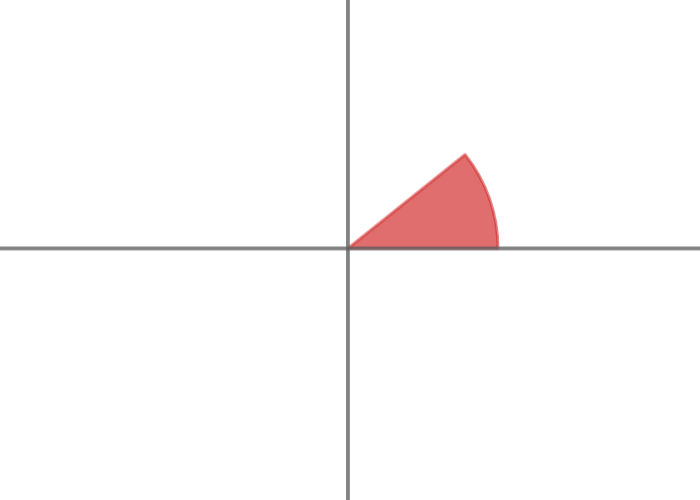
\includegraphics[width=1.35cm]{Image/Angles/aigu.PNG} & 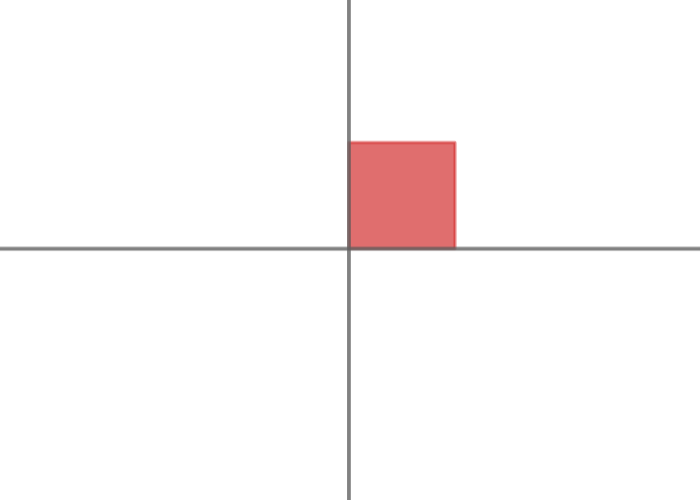
\includegraphics[width=1.35cm]{Image/Angles/droit.PNG} & 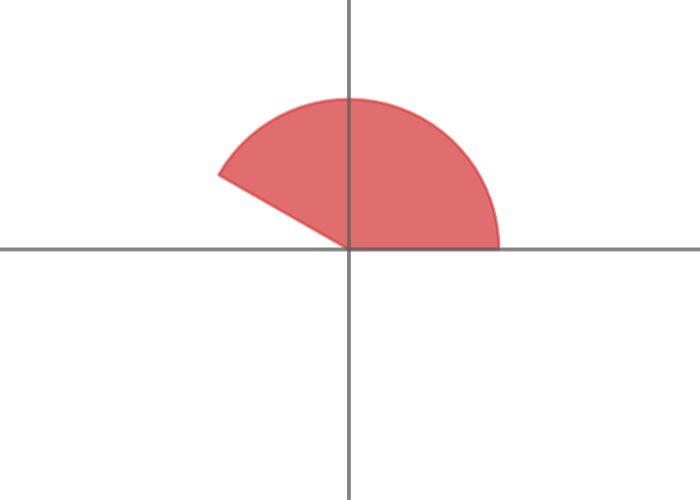
\includegraphics[width=1.35cm]{Image/Angles/obtu.PNG} & 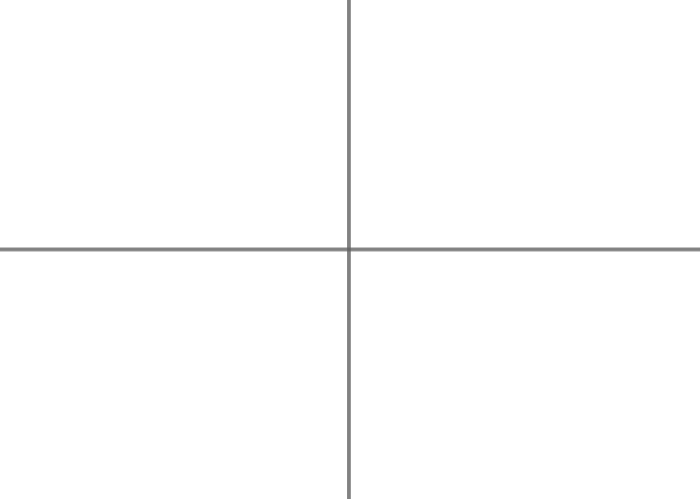
\includegraphics[width=1.35cm]{Image/Angles/angle_nul.PNG} & 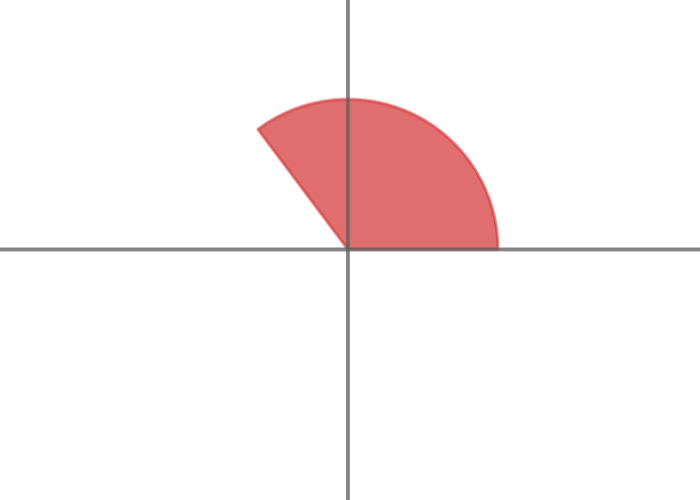
\includegraphics[width=1.35cm]{Image/Angles/saillant.PNG} & 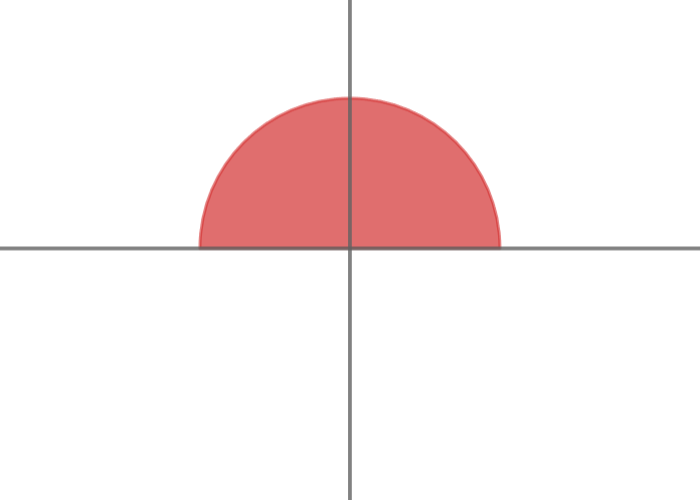
\includegraphics[width=1.35cm]{Image/Angles/plat.PNG} & 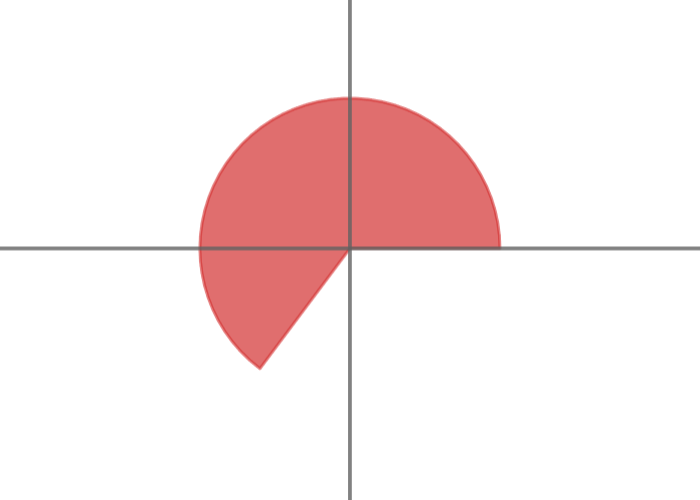
\includegraphics[width=1.35cm]{Image/Angles/rentrant.PNG} & 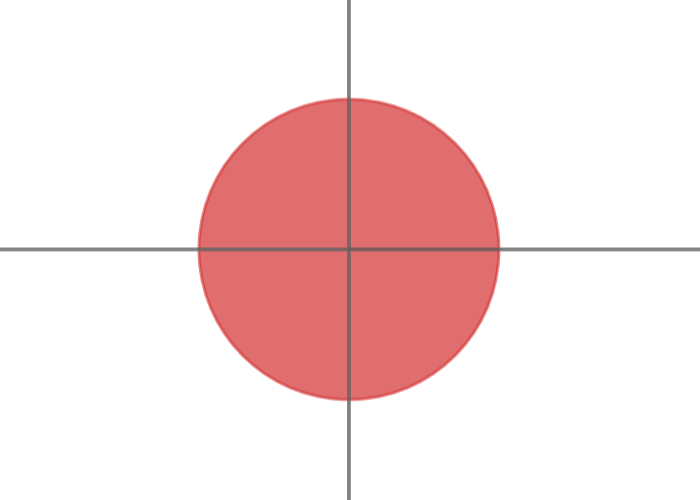
\includegraphics[width=1.35cm]{Image/Angles/plein.PNG} \\
			\hline
			] $0^\circ ; 90^\circ$[                               & \(90^\circ\)                                           & ] \(90^\circ ; 180^\circ\)[                           & \(0^\circ\)                                                & ] \(0^\circ ; 180^\circ\)[                                & \(180^\circ\)                                         & ]\(180^\circ ; 360^\circ\)[                               & \(360^\circ\)                                          \\
					\hline
			]$0 ; \frac{\pi}{2}$[                                 & $\frac{\pi}{2}$                                        & ]$\frac{\pi}{2} ; \pi$[                               & $0$                                                        & ]$0 ; \pi$[                                               & $\pi$                                                 & ]$\pi ; 2\pi$[                                            & $2\pi$                                                 \\
			\hline
		\end{tabular}
	}
\end{center}

Avec ce tableau, on peut facilement comprendre comment fonctionne cette mesure.
On se base sur un \emph{angle plein} (définit comme mesurant \(360^\circ\), \(2\pi\) rad ou \(400\) gr),
puis on divise cet angle plein en fonction de l'angle que l'on souhaite mesuré.
Ainsi, un \emph{angle droit} qui correspond à un quart d'un angle plein,
mesurera \(90^\circ\), \(\frac{\pi}{2}\) rad ou \(100\) gr.

Comme on peut le remarquer, les différentes unités varie uniquement sur le choix de la mesure
d'un angle plein, et chaque choix apporte certains avantages. En degré, l'intérêt du nombre 360 s'explique
par la multitude de diviseur dont ce dernier dispose. En radian, $2\pi$ correspond au périmètre
d'un cercle de rayon unitaire, ce qui est (en résumé) très cohérent mathématiquement. En grade,
un angle droit mesure 100, nombre étant facilement manipulable.

\subsubsection*{Conversion d'une unité à une autre}

\begin{center}
	\renewcommand{\arraystretch}{1.5}
	\begin{tabular}{|c|c||c|c|}
		\hline
		\textbf{Conversion} & \textbf{Formule} & \textbf{Constante} & \textbf{$\log_{10}(\text{Constante})$} \\
		\hline
		\textcolor{Red}{$x$ degré} $\Rightarrow$ \textcolor{Blue}{$y$ radian} & $y = x \times \frac{2 \pi}{360} = x \times \frac{\pi}{180}$ & $\frac{\pi}{180} \approx \numprint{0,017 453}$ & $-\numprint{1.758122632}$\\
		\textcolor{Blue}{$x$ radian} $\Rightarrow$ \textcolor{Red}{$y$ degré} & $y = x \times \frac{360}{2 \pi} = x \times \frac{180}{\pi}$ & $\frac{180}{\pi} \approx \numprint{57,295 78}$ & $+\numprint{1.758122632}$\\
		\hline
		\textcolor{Red}{$x$ degré} $\Rightarrow$ \textcolor{Green}{$y$ grade} & $y = x \times \frac{400}{360} = x \times \frac{10}{9}$ & $\frac{10}{9} = 1,111...$ & $+\numprint{0.045757490}$\\
		\textcolor{Green}{$x$ grade} $\Rightarrow$ \textcolor{Red}{$y$ degré} & $y = x \times \frac{360}{400} = x \times 0,9$ & $0,9$ & $-\numprint{0.045757491}$ \\
		\textcolor{Blue}{$x$ radian} $\Rightarrow$ \textcolor{Green}{$y$ grade} & $y = x \times \frac{400}{2 \pi} = x \times \frac{200}{\pi}$ & $\frac{200}{\pi} \approx \numprint{63,661 98}$ & $+\numprint{1.803880123}$ \\
		\textcolor{Green}{$x$ grade} $\Rightarrow$ \textcolor{Blue}{$y$ radian} & $y = x \times \frac{2 \pi}{400} = x \times \frac{\pi}{200}$ & $\frac{\pi}{200} \approx \numprint{0,0157 08}$ & $-\numprint{1.803 880 123}$\\
		\hline
	\end{tabular}
\end{center}
Valeurs approchées et Logarithmes des constantes : …

\newpage

\subsubsection*{Propriétés}

\paragraph*{Angles complémentaires}

Deux angles sont \emph{complémentaires} si une fois réunis, ils forment ensemble un \textit{angle droit}.

\paragraph*{Angles supplémentaires}

Deux angles sont \emph{supplémentaires} si une fois réunis, ils forment ensemble un \textit{angle plat}.

\paragraph*{Angles explémentaires}

Deux angles sont \emph{explémentaires} si une fois réunis, ils forment ensemble un \textit{angle plein}.

\subsubsection*{Bissectrice}

La \emph{bissectrice} d'un angle est une droite séparant un angle en deux secteurs d'angle égaux.

Pour savoir comment tracer une bissectrice, rendez-vous page n°\pageref{tracer_mediatrice_bissectrice}.




\subsubsection*{Notation d'un angle}

La notation des angles est, en revanche, un peu plus technique.
Prenons un exemple pour bien comprendre :

\begin{center}
	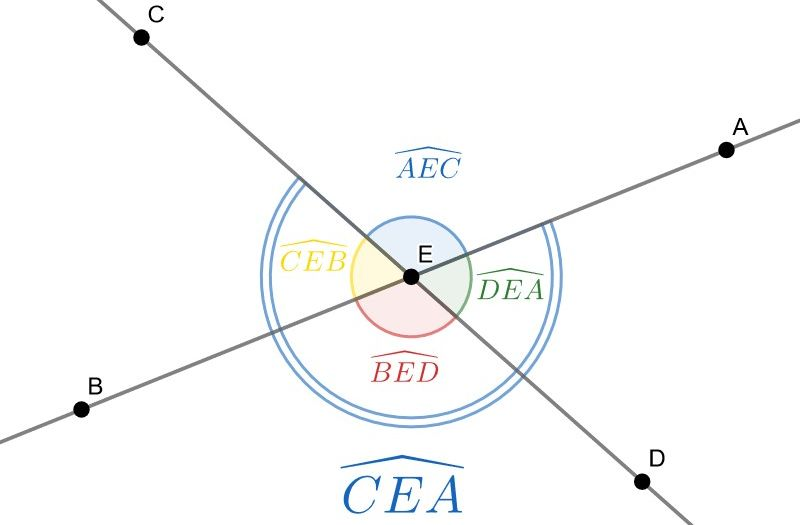
\includegraphics[width=10cm]{Image/Angles/notation_angle.jpg}
\end{center}

Voici deux droites $(AB)$ et $(CD)$ se croisant au point E, le croisement forme 4 angles différents,
il sont représentés en 4 couleurs différentes.

Pour distinguer les angles entre eux, un sens de rotation a été définit,
ce sens est le sens inverse des aiguilles d'une montre.

Ce qui signifie que l'angle bleu, formé entre les demi-droites $[EA)$ et $[EC)$,
est angle qui commence à partir de $[EA)$ et qui termine une fois arrivée à $[EC)$.
On note donc cet angle $\widehat{AEC}$. En revanche, l'angle formé entre $[EC)$ et $[EA)$
(dans cet ordre là), est représenté par un double arc de cercle, et on le note $\widehat{CEA}$,
car il débute sur $[EC)$ et il se termine au niveau de $[EA)$.

Avec cette méthode, on peut nommer tous les autres angles :
le jaune est $\widehat{CEB}$, le rouge est $\widehat{BED}$ et le vert se note $\widehat{DEA}$.

Alternativement, il est possible de désigner un angle par une autre notation, classiquement, en utilisant les
lettres grecs\footnote{L'ensemble des symboles utilisés en Mathématique sont présenté à la page n°\pageref{symboles_math}.}.



\newpage

\subsection{Repère cartésien orthonormé}

La première étape pour faire de la géométrie dans les règles de l'art,
est d'utiliser un repère cartésien orthonormé.
Ce repère sert à placer les points dans notre plan.

\medbreak

Pour le construire, il faut tracer deux droites perpendiculaires entre-elles.
Les droites du repère se croisent en un point généralement appelé $O$
(La lettre “O” en majuscule). Puis, il faut graduer ces droites,
c'est-à-dire placer sur ces dernières, de manière régulière, des points associés à des valeurs,
ces valeurs sont croissantes en allant de la gauche vers la droite et en allant du bas vers le haut.

Ces droites graduées sont maintenant les axes du repère.
L'axe horizontal est l'axe des abscisses et le vertical est l'axe des ordonnées.
Ces axes nous permettent de donner un couple de valeurs à chaque point du plan.
Ce couple est la seul information nécessaire pour localiser un point du plan.
Dans ce couple, on note en premier l'abscisse du point, puis son ordonné.
Et ce couple est appelé la \emph{coordonnée du point}, de plus comme nous sommes
dans un repère cartésien, ce couple est la \emph{coordonnée cartésienne}
\footnote{Il existe d'autres systèmes de coordonnées pour repérer des points dans un plan,
comme le \emph{système de coordonnées polaires}, où un point $A$ est à une distance connue de
l'origine du repère, et est placé de manière à ce que la demi-droite $[OA)$
forme avec l'axe des abscisses positives un angle connu.
Ainsi, dans ce système de coordonnée, un point n'est pas placé à l'aide de deux distances,
mais avec une distance et un angle.} du point.

\medbreak

Et enfin, les axes sont associés à des lettres, très pratiques dans de nombreux cas.
Généralement, l'axe des abscisses est l'axe des $x$ et le second est l'axe des $y$.

\medbreak

Par exemple, dans le repère suivant, le point A à pour coordonnée $(x_A ; y_A)$,
avec $x_A = 3$ et $y_A = 2$ et le point B se trouve à la coordonnée $(-1 ; 3)$.

\begin{center}
	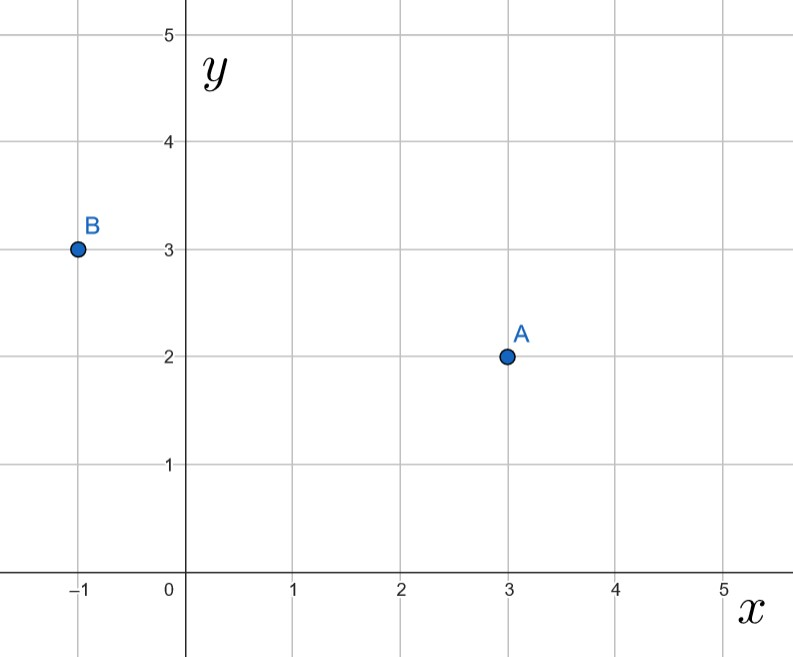
\includegraphics[width=10cm]{Image/repere_cartesien_orthonorme.jpg}
\end{center}

En plus des axes, on retrouve une grille étant tracé plus finement,
cette grille n'est pas toujours présente,
mais elle est très utile pour placer précisément les points nous étant utiles.

\newpage

% -------------------------------------------------------------

\section{Les formes géométriques planes}

Les formes géométriques planes (constructibles dans un plan) 
les plus classiques que l'on retrouve dans cette discipline
sont les cercles et les polygones.

\medbreak

Ces formes sont caractérisables par leur périmètre et leur aire :

\vspace{-0.2cm}

\subparagraph*{Périmètre} Ligne délimitant le contour d'une forme géométrique plane.
On nomme généralement sa longueur $p$.

\vspace{-0.2cm}

\subparagraph*{Aire} Valeur mesurant la portion de surface limitée par le périmètre d'une figure.
On nomme généralement cette grandeur $\mathcal{A}$. L'aire se mesure comme étant un multiple d'une surface
de référence, dans notre repère cartésien orthonormé, cette surface de référence correspond à l'aire
d'un carré dont ses côtés mesurent 1.

Si l'unité de mesure des longueur est le mètre (m), alors l'unité de mesure des surface sera
cette unité de longueur multipliée par elle-même, ici on obtient le mètre-carré (m²).

\medbreak

Par simplification, on confond le périmètre (le véritable, celui définit précédemment) avec la longueur de ce dernier.
D'ailleurs, c'est aussi le cas pour beaucoup d'autres caractéristiques,
on confond souvent le concept mathématique et la mesure de celui-ci.

Il est par exemple assez commun de dire que telle figure à un périmètre de 10,
que tel cercle à un rayon de 2, ce qui implique que son diamètre vaut 4.

\medbreak

Nous allons maintenant nous attarder sur l'étude des figures en elles-mêmes,
nous commencerons par le \emph{cercle} (page suivante), puis par les \emph{polygones} (page n°\pageref{polygones}).

En suite nous nous attarderons sur 2 familles de polygones importantes,
ce sont les \emph{triangles} (page n°\pageref{triangles}) et les \emph{quadrilatères} (page n°\pageref{quadrilateres}).

\newpage

\subsection{Le cercle}

Un cercle est une forme géométrique, qui est formée de l'ensemble des points équidistants
à point choisi, ce point sera le centre du cercle.
La distance séparant les points formant le cercle de son centre est le rayon du cercle,
souvent noté $r$.

Voici un cercle de centre O aux coordonnées $(0;0)$, et ayant un rayon égal à 3 :

\begin{center}
	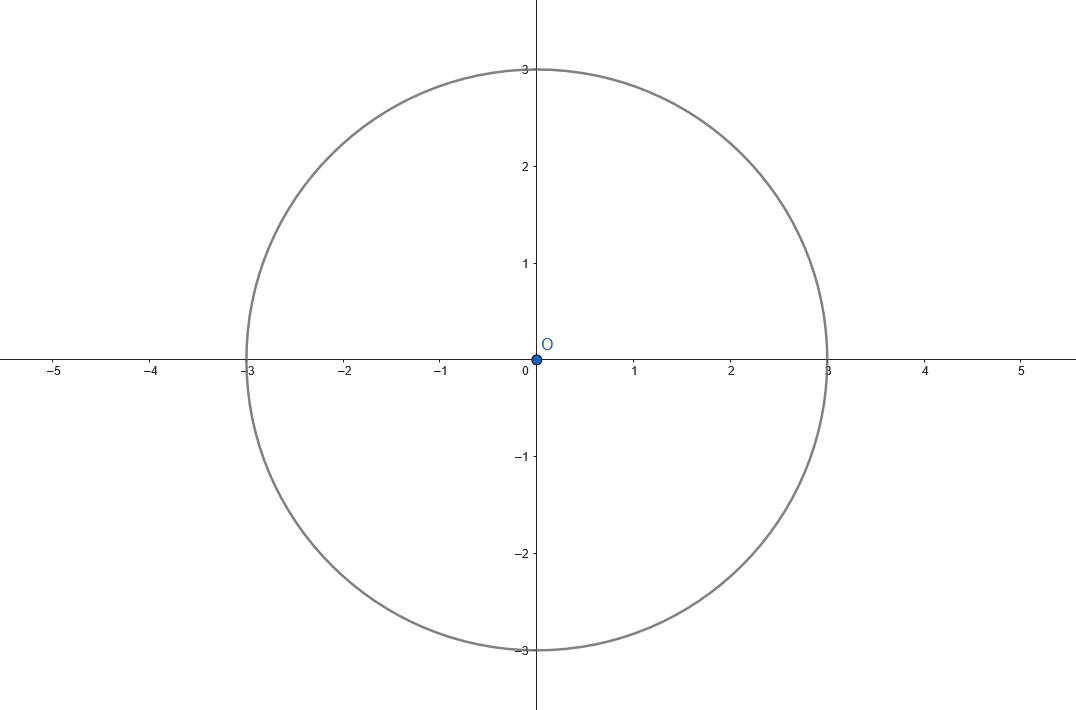
\includegraphics[width=7.5cm]{Image/cercle_centre_O_rayon_3.png}
\end{center}

Pour construire une représentation d'un cercle,
il faut représenter tous les points éloignés de la même distance par rapport au point central.
Cela peut être fait à l'aide d'une corde bien tendue entre un bâton et un crayon,
on place le bâton là où l'on souhaite que se trouve le centre du cercle,
puis il faut faire tourner le crayon autour du bâton en faisant attention à ne pas modifier
la distance entre le crayon et le bâton.

Afin de ne pas avoir à surveiller la tension de la corde, l'homme inventa le \emph{compas},
un outil disposant de deux pointes éloignables, la première joue le rôle du bâton,
en se plaçant au centre du cercle, et la seconde trace le cercle.
Comme l'outil est rigide, il rend la construction de cercle très facile.

\medbreak

On peut définir différentes caractéristiques du cercle à partir de son rayon r,
et grâce la constante $\pi$ :

\medbreak

\begin{itemize}
	\item[•] Son \emph{diamètre} $d_{cercle}$, qui correspond à sa largeur maximale.
	      Avec $r$ le rayon du cercle, on a $d_{cercle} = 2 \times r$.
	      \smallbreak
	\item[•] Son \emph{périmètre} $p_{cercle} = d \times \pi = 2 \cdot r \times \pi = 2 \pi r$. (Moyen mnémotechnique : 2 pierres)
	      \smallbreak
	\item[•] Son \emph{aire} $\mathcal{A}_{cercle} = \pi \times r^2$.
\end{itemize}

\medbreak

Les démonstrations de ces formules sont présentées en bas de page.\footnote{
	Tous les diamètres du cercle passent par son centre.
	Ainsi, on peut découper chacun de ces diamètres en deux parties égales,
	ces parties sont des segments liant le centre du cercle et les point le composant,
	on remarque alors que ces parties sont des rayons du cercle.
	Donc, le diamètre d'un cercle est composé de deux de ses rayons accolés. On en conclue que $d = 2 \times r$.}$^{, }$\footnote{
	La formule du périmètre n'a pas de démonstration,
	car c'est cette formule qui définit la constante $\pi$.
	On s'est dans un premier temps rendu compte que tous les cercles étaient semblables,
	à un agrandissement ou une réduction près, ainsi nous en déduisîmes que le périmètre d'un cercle
	dépendait uniquement de son diamètre.
	Donc, nous avons créé cette
	formule et la constante
	$\pi$.}$^{, }$
\footnote{
	La démonstration de cette dernière est un peu plus technique,
	vous pouvez la retrouver en Annexe (page n°\pageref{demo_formule_aire_cercle}).}

\subparagraph*{La constante $\mathbb{\pi}$}

$\pi$ (prononcé “pi” (comme le pis d'une vache)) est la première lettre du mot
\begin{otherlanguage*}{greek}
	περιφέρεια,
\end{otherlanguage*}
signifiant périmètre en grec.

Mais cette lettre est aujourd'hui bien plus associé à la constante mathématique
qu'à la notion de périmètre.
Cette constante est définit comme étant le rapport entre
le périmètre du cercle et son diamètre. Mathématiquement
voilà ce que cela donne : $$\pi = \frac{p_{cercle}}{d} = \frac{p_{cercle}}{2 \times r}$$

En passant le dénominateur à gauche,
on retrouve la formule utilisée pour calculer le périmètre d'un cercle,
car c'est ce calcul qui a amené les grecs à inventer la constante $\pi$.
Pour en savoir plus, l'histoire de cette constante est détaillée en Annexe (page n°\pageref*{histoire_de_pi}).

\medbreak

Mais malheureusement, $\pi$ n'a pas une valeur exacte,
car il a d'une infinité de décimale. On connais à l'heure où j'écrits ces lignes,
l'on connais les cent mille milliards premières de décimale de $\pi$\footnote{
	Le 9 juin 2022, le record du nombre de décimale calculée est battu par Emma Haruka Iwao,
	calculant cette fois cent mille milliards de décimales,
	grâce aux puissants ordinateurs de Google.}.%[https://cloud.google.com/blog/products/compute/calculating-100-trillion-digits-of-pi-on-google-cloud?hl=en]

Heureusement, nous n'avons pas besoin d'une telle précision pour
Utiliser cette constante en pratique. Cette constante est tellement importante
et iconique que le grand public connaît une approximation de celle-ci,
beaucoup de personnes savent que $\pi \approx 3,14$.

Cette approximation n'est pas parfaite, mais elle est largement
satisfaisante dans beaucoup d'applications, pour en savoir plus, rendez-vous en Annexe (page n°\pageref*{approximations_pi}).

On peut aller plus loin en rajoutant quelques décimales $\pi = \numprint{3,141592653589793}...$

\medbreak

Mais de toute façon, en Mathématique, on n'utilise que des valeurs exactes !
Donc finalement, peu importe le nombre de décimales de $\pi$ connues, car nous allons utiliser
directement $\pi$ dans nos expressions. L'aire d'un cercle de rayon 3 vaut donc $\pi \times 3^2 = 9 \pi$, et
on ne va pas chercher à obtenir une valeur approchée de $9 \pi$, à part évidemment si
l'on souhaite appliquer dans le monde réel les résultats obtenus !

\subparagraph*{Propriétés} Une ligne et un cercle sont \emph{tangents} entre eux,
s'ils se touchent en un seul point.

\newpage

\subsection{Les polygones} \label{polygones}

Un polygone est une forme géométrique constituée d'un certain nombre de points
(qui sont les \emph{sommets} du polygone) reliés par des segments (les \emph{arêtes}
ou les \emph{côtés} du polygone).

\medbreak

Les polygones sont classés en fonction de leur nombre de côtés\footnote{
	La nomenclature des polygones est présentée en Annexe, à la page \pageref{nomenclature_polygone_polyèdre}.
} :

\begin{center}
	\begin{tabular}{|c|c|c|c|c|}
		\hline
		\textit{3 côtés}                  & \textit{4 côtés}  & \textit{5 côtés}  & \textit{6 côtés}  & \textit{7 côtés}                    \\

		Triangle                          & Quadrilatère      & Pentagone         & Hexagone          & Heptagone                           \\
		\hline
		\hline
		\textit{8 côtés}                  & \textit{9 côtés}  & \textit{10 côtés} & \textit{11 côtés} & \textit{12 côtés}                   \\

		Octogone                          & Ennéagone         & Décagone          & Hendécagone       & Dodécagone                          \\
		\hline
		\hline
		\textit{20 côtés}                 & \textit{30 côtés} & \textit{40 côtés} & \textit{50 côtés} & \textit{100 côtés}                  \\

		\phantom{cc}Icosagone\phantom{cc} & Triacontagone     & Tétracontagone    & Pentacontagone    & \phantom{cc} Hectogone \phantom{cc} \\
		\hline
	\end{tabular}
	\medbreak

	\textit{Les polygones ayant 1 ou 2 côtés ne sont pas constructibles sur un plan.}

\end{center}

\paragraph*{Nommer un polygone}

Un polygone est une figure géométrique composée de plusieurs points.
Pour désigner cette figure, 
on nomme les points en suivant les côtés du polygone,
dans n'importe quel sens,
en commençant par n'importe quel sommet.

Il est important de bien suivre les côtés du polygone, 
pour bien pouvoir distinguer ces deux polygones :

\begin{center}
	\begin{tabular}{ccc}
		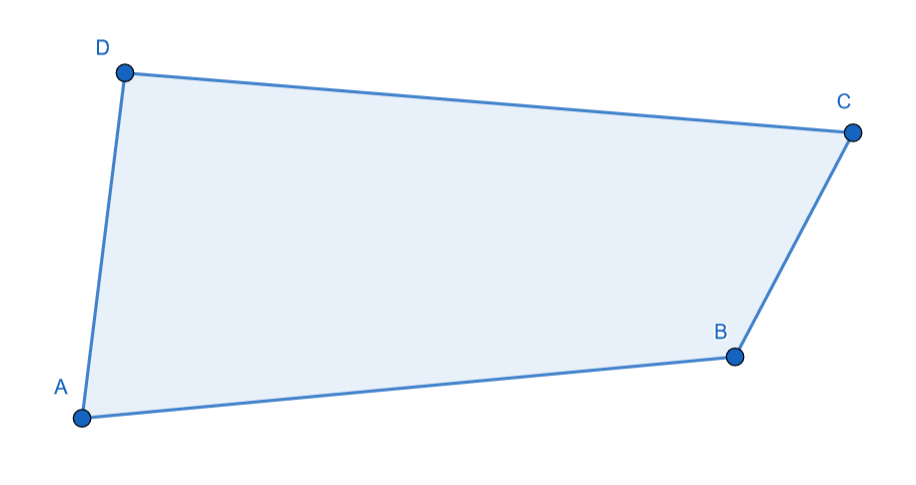
\includegraphics[width=6cm]{Image/Polygone ABCD.png} &               & 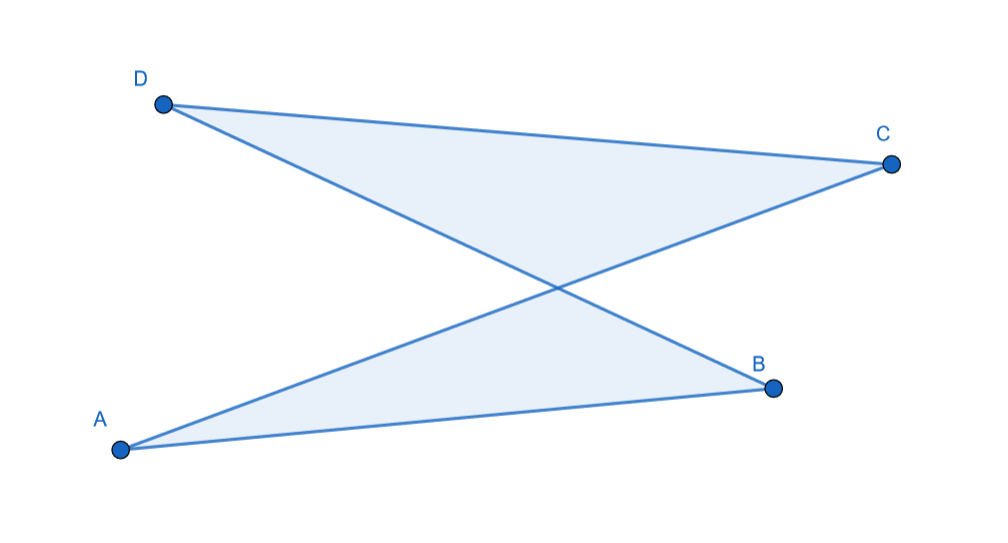
\includegraphics[width=6cm]{Image/Polygone ABDC.png} \\
		\textit{Quadrilatère $ADCB$, $DCBA$ ou $ABCD$}       & \phantom{cou} & \textit{Quadrilatère $ACDB$, $DBAC$ ou $ABDC$}                         \\
	\end{tabular}
\end{center}

\paragraph*{Angles intérieurs et extérieurs}

On appelle \emph{angle interne} d'un polygone \textit{simple}
l'angle formé en un sommet de ce polygone,
à l'intérieur de celui-ci,
par les deux côtés de ce polygone adjacents en ce sommet.

Pour obtenir l'angle externe d'un polygone en un sommet,
on choisit l'un des deux côtés adjacents en ce sommet et
on prolonge l'autre côté à partir du sommet considéré.
L'angle entre le côté fixé et le prolongement de l'autre côté adjacent
s'appelle l'\emph{angle externe}.
Comme il y a deux possibilités dans le choix du côté adjacent fixé,
il y a deux manières de construire l'angle externe en un sommet.
Ces deux angles étant opposés par le sommet, ils ont la même mesure.

Ainsi par exemple, dans un triangle équilatéral,
tous ses angles intérieurs mesurent $60^\circ$ et
tous ses angles extérieurs mesurent $120^\circ$.

\textit{La plupart du temps, on utilise uniquement les angles intérieurs des polygones.}

\paragraph*{Polygone simple ou croisé}

Un polygone est dit \emph{croisé} si dans celui-ci, deux côtés non adjacents se croisent.
Si aucun de ses côtés ne se croisent, alors le polygone est \emph{simple} (ou \textit{non croisé}).

Un polygone \textit{simple} forme une courbe de Jordan\footnote{
	Pour en savoir plus,
	rendez-vous en annexe (à la page n°\pageref*{courbe_Jordan}).},
qui délimite une partie bornée du plan, appelée son intérieur.
On appelle \emph{aire} d'un polygone simple l'aire de son intérieur.

\begin{itemize}
	\item[•] Généralement, on s'intéresse seulement aux polygones \textit{simples}.
	\item[•] Les triangles ne peuvent pas être croisés.
\end{itemize}

\paragraph*{Convexité}

Un objet géométrique est \emph{convexe} si,
pour n'importe quel couple de points choisi,
le segment rejoignant ces points reste contenu dans l'objet.
Si avec un seul couple, le segment sort de l'objet,
alors l'objet est \emph{concave}.

Un polygone est \textit{simple},
si tous ses angles sont \textit{saillants} \textbf{ou}
s'il n'existe pas de segment joignant deux sommets de ce polygone étant à l'extérieur de celui-ci.

\paragraph*{Polygone régulier}

Un \emph{polygone régulier} est un \emph{équilatéral}
(tous ses côtés ont la même longueur) et \emph{équiangle}
(tous ses angles ont la même mesure).

Les polygones réguliers peuvent être convexes ou concaves.
Les polygones réguliers convexes sont des polygones étoilés\footnote{
	Ce type de polygone est présenté plus en détail à la page n°\pageref*{polygone_etoile}
}.

Un polygone régulier a autant d'axes de symétrie que de côtés.

Dans les polygones réguliers concaves, les angles intérieurs sont tous égaux.
Ainsi, ces angles valent la \textit{somme des angles intérieurs du polygone} divisée par le nombre d'angles intérieurs.

Pour un triangle équilatéral,
la somme des angles intérieurs vaut $180^\circ$,
donc chaque angle intérieur $\alpha$ est égal à $\frac{180^\circ}{3} = 60^\circ$.

\begin{center}
	\begin{tabular}{cccccc}
		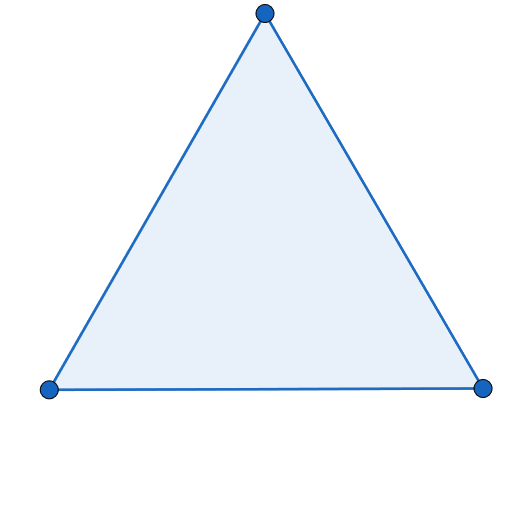
\includegraphics[width=2cm]{Image/Polygones Reguliers/Triangle equilateral.png} &
		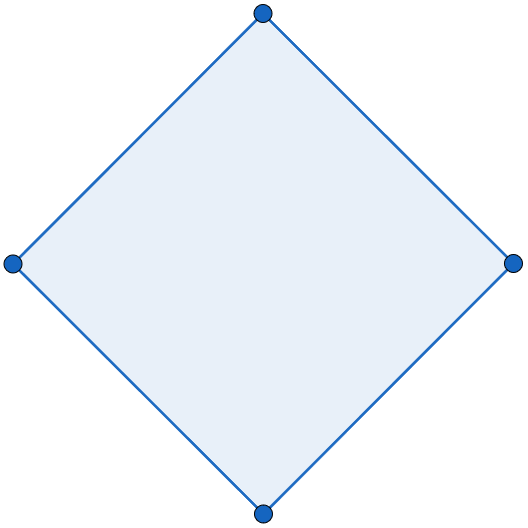
\includegraphics[width=2cm]{Image/Polygones Reguliers/Carre.png}                &
		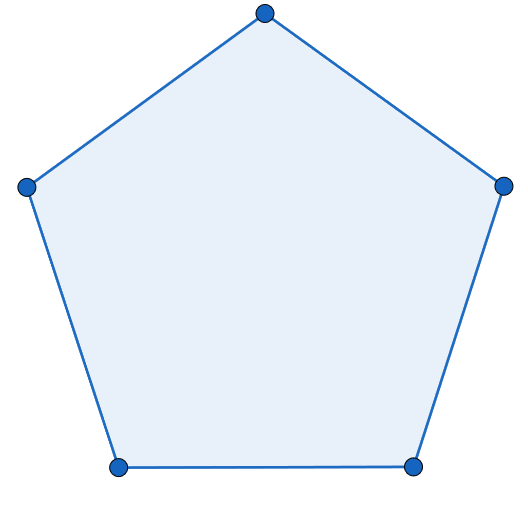
\includegraphics[width=2cm]{Image/Polygones Reguliers/Pentagone regulier.png}   &
		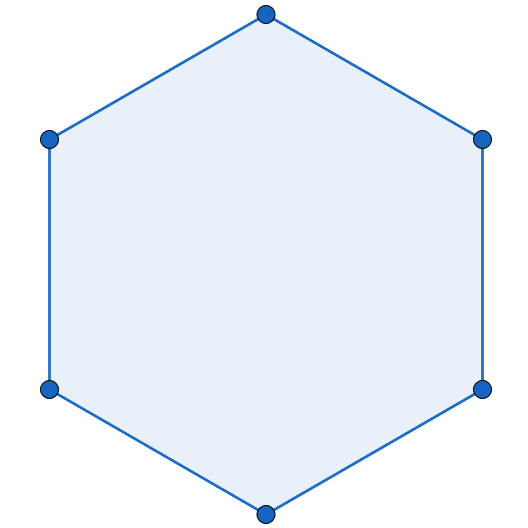
\includegraphics[width=2cm]{Image/Polygones Reguliers/Hexagone regulier.png}    &
		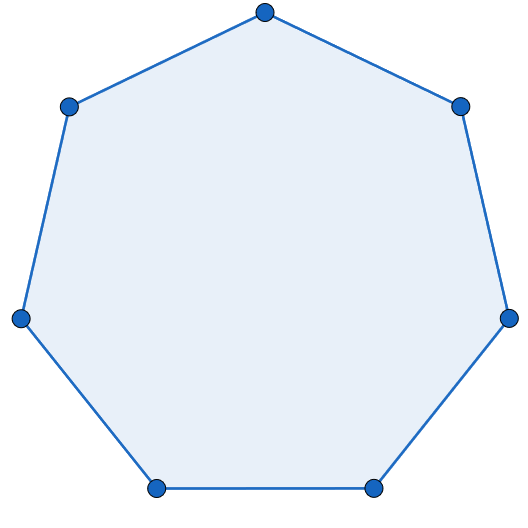
\includegraphics[width=2cm]{Image/Polygones Reguliers/Heptagone regulier.png}   &
		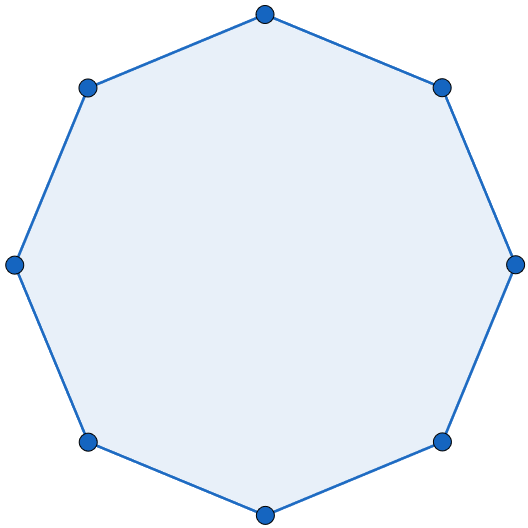
\includegraphics[width=2cm]{Image/Polygones Reguliers/Octogone regulier.png}    \\

		\textit{Triangle}    & \multirow{2}{*}{\textit{Carré}} & \textit{Pentagone} & \textit{Hexagone} & \textit{Heptagone} & \textit{Octogone} \\
		\textit{équilatéral} &                                 & \textit{régulier}  & \textit{régulier} & \textit{régulier}  & \textit{régulier} \\

		& & & & & \\

		\multicolumn{1}{l}{$\alpha =  60^\circ$}          &
		\multicolumn{1}{l}{$\alpha =  90^\circ$}          &
		\multicolumn{1}{l}{$\alpha = 108^\circ$}          &
		\multicolumn{1}{l}{$\alpha = 120^\circ$}          &
		\multicolumn{1}{l}{$\alpha \approx 128.57^\circ$} &
		\multicolumn{1}{l}{$\alpha = 135^\circ$}          \\

		\multicolumn{1}{l}{$\alpha = \frac{  \pi}{3} \text{ rad}$} &
		\multicolumn{1}{l}{$\alpha = \frac{  \pi}{2} \text{ rad}$} &
		\multicolumn{1}{l}{$\alpha = \frac{3 \pi}{5} \text{ rad}$} &
		\multicolumn{1}{l}{$\alpha = \frac{2 \pi}{3} \text{ rad}$} &
		\multicolumn{1}{l}{$\alpha = \frac{5 \pi}{7} \text{ rad}$} &
		\multicolumn{1}{l}{$\alpha = \frac{3 \pi}{4} \text{ rad}$} \\

		\multicolumn{1}{l}{$\alpha \approx 66.67 \text{ gr}$}  &
		\multicolumn{1}{l}{$\alpha = 100 \text{ gr}$}          &
		\multicolumn{1}{l}{$\alpha = 120 \text{ gr}$}          &
		\multicolumn{1}{l}{$\alpha \approx 133.33 \text{ gr}$} &
		\multicolumn{1}{l}{$\alpha \approx 142.86 \text{ gr}$} &
		\multicolumn{1}{l}{$\alpha = 150 \text{ gr}$}          \\
	\end{tabular}
\end{center}

\paragraph*{Somme des angles intérieurs d'un polygone}

Notons $n$ le nombre de côtés d'un polygone quelconque. La somme des angles intérieurs
du polygone vaut\footnote{Ces formules sont
	démontrées en Annexe, à la page n°\pageref*{demo_formule_lien_somme_angle_nb_cote}.}:

\begin{center}
	\begin{tabular}{ccccc}
		$180 \times (n-2)$       &               & $\pi \times (n-2)$        &               & $200 \times (n-2)$       \\
		\textit{Angles en degré} & \phantom{ccc} & \textit{Angles en radian} & \phantom{ccc} & \textit{Angles en grade} \\
	\end{tabular}
\end{center}

\medbreak

\paragraph*{Périmètre d'un polygone}

La longueur du périmètre d'un polygone est facile à obtenir,
elle est égale à la somme des longueurs de tous les côtés du polygone.

\paragraph*{Axes de symétrie}

Traçons une figure sur notre plan,
si lorsque l'on plie le plan en suivant un axe donné,
notre figure se superpose parfaitement,
alors cet axe est un \emph{axe de symétrie de la figure}.

Cette transformation du plan est une \textbf{symétrie axiale}.

\subparagraph*{Cas des polygones}

Dans un polygone non croisé, les axes de symétrie (s'ils existent),
sont forcément des \emph{médiatrices} ou des \emph{bissectrices}, de plus,
si cet axe est une bissectrice, alors les côtés l'encadrant doivent être de même
longueur.\footnote{
	Je nommerai ce type de bissectrice, des \emph{bissectrices isocèles}.
}$^\text{,}$\footnote{
	La démonstration est disponible en Annexe, à la page n°\pageref*{demo_axes_symétrie_polygone}
}

\paragraph*{Côtés prolongés}

Les droites passant par les côtés d'un polygone sont appelées
les \emph{côtés prolongés} de ce polygone.


\paragraph*{Diagonales}

Une \emph{diagonale} d'un polygone est un segment qui joint deux sommets non consécutifs,
c'est-à-dire un segment joignant deux sommets et n'étant pas un côté du polygone.

Un polygone à $n$ côtés possède ainsi $\binom{n}{2} - n = \frac{n(n-3)}{2}$ diagonales.

\newpage

\subsection{Les Triangles} \label{triangles}

Les triangles sont des polygones à trois côtés et la somme de leurs angles
intérieurs vaut $180^\circ$, $\pi$ rad ou $200$ gr.
%[Triangle](https://fr.wikipedia.org/wiki/Triangle)

\subsubsection{Classification des Triangles}

Il existe différents types de triangles,
ils sont classés en fonction des longueurs de leurs côtés et de leurs angles.

\medbreak

Voici les différents types de triangles :

\medbreak

\begin{itemize}
	\item[•] \textbf{Triangle équilatéral} :
	      Les trois côtés du triangle équilatéral ont la même longueur,
	      ce qui fait que tous les angles intérieurs de ce triangle mesurent 60°
	      (ou $\frac{\pi}{3}$ rad).\footnote{
		      \textbf{Construction} : Tracez un segment d'une longueur $l$ choisie,
		      puis tracez deux cercles de rayon $l$, ayant pour centre chacune des deux extrémités du segment.
		      Ces cercles se croisent en deux points,
		      pour obtenir un triangle équilatéral,
		      reliez l'un d'entre-eux aux extrémités du segment initial.

		      Les propriétés des triangles équilatéraux sont démontrées en Annexe, à la page \pageref{propriete_triangle_equilateral}.
			  \smallbreak
	      }
		  \medbreak
	\item[•] \textbf{Triangle isocèle} : Au moins deux côtés du triangle isocèle ont la même longueur,
	      ce qui engendre que les angles opposés aux côtés égaux sont également égaux.\footnote{
		      \textbf{Construction} : Tracez un segment d'une longueur $a$ choisie,
		      puis tracez deux cercles de rayon $b$, ayant pour centre chacune des deux extrémités du segment.
		      Ces cercles se croisent en deux points,
		      pour obtenir un triangle isocèle,
		      reliez l'un d'entre-eux aux extrémités du segment initial.

			  Les propriétés des triangles isocèles sont démontrées en Annexe, à la page \pageref{propriete_triangle_isocele}.
		      \smallbreak
		  } Le sommet où les deux côtés égaux se rejoignent est le \emph{sommet principal}.
		  Le côté opposé au sommet principal est la \emph{base} du triangle.
		  \medbreak
	\item[•] \textbf{Triangle scalène} : Aucun des côtés du triangle scalène n'a la même longueur,
	      et il en est de même pour les angles, ils sont forcément tous différents. \footnote{
		  	 Les propriétés des triangles scalènes sont démontrées en Annexe, à la page \pageref{propriete_triangle_scalene}.
	      }

	      \medbreak\medbreak\medbreak

	\item[•] \textbf{Triangle rectangle} : Un triangle rectangle a un angle droit.
	      Le côté opposé à l'angle droit est appelé l'\emph{hypoténuse},
	      et les côtés adjacents à l'angle droit sont appelés \emph{cathètes} (ou simplement \textit{côtés adjacents}).
		  \medbreak
    \item[•] \textbf{Triangle obtusangle \textit{(ou amblygone)}} : Un triangle obtusangle a un angle obtus.
	      Les deux autres angles seront nécessairement aigus.
		  \medbreak
	\item[•] \textbf{Triangle acutangle \textit{(ou oxygone)}} : Un triangle acutangle a trois angles aigus.

	\medbreak\medbreak\medbreak

	\item[•] \textbf{Triangle quelconque} : Ce type de triangle n'a aucune propriété particulière. 
	On appelle \textit{quelconque} un triangle générique, n'ayant aucune propriété en particulier. 
\end{itemize}

\bigbreak

Chaque triangle rentre dans au moins 2 des 6 types de triangles présentés plus haut.
Une en fonction des longueurs de ses côtés, l'autre en fonction de la mesure de ses angles.

De plus, si un triangle $ABC$ est isocèle et a comme sommet principal $B$, on dira qu'il est \textit{isocèle en $B$}.
Il en est de même pour les triangles \textit{rectangles} et \textit{obtusangles}, 
on précise (si l'information est connue) dans la dénomination son sommet important.

\paragraph*{Représentation des différents types de triangles}

\begin{center}
	\makebox[\textwidth][c]{
		\begin{tabular}{ccc|ccc}
			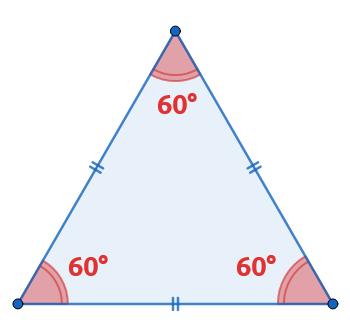
\includegraphics[width=2.2cm]{Image/Triangles/triangle_equilateral_complet.png} &
			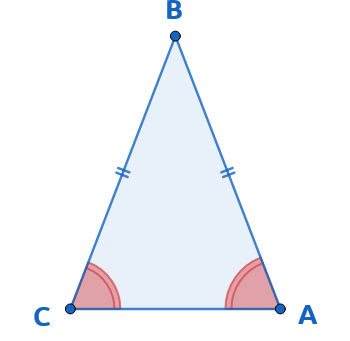
\includegraphics[width=2.2cm]{Image/Triangles/triangle_isocele_complet.png}     &
			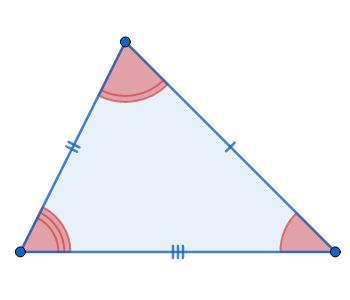
\includegraphics[width=2.5cm]{Image/Triangles/triangle_scalene_complet.png}     &
			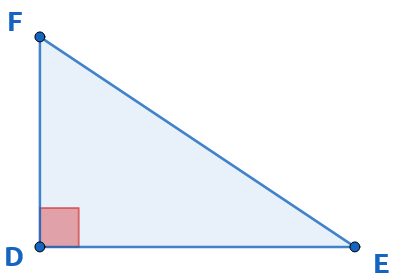
\includegraphics[width=2.5cm]{Image/Triangles/triangle_rectangle_complet.png}   &
			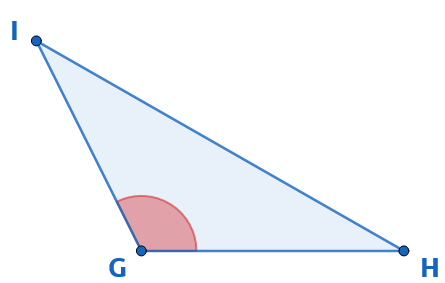
\includegraphics[width=3cm  ]{Image/Triangles/triangle_optusangle_complet.png}  &
			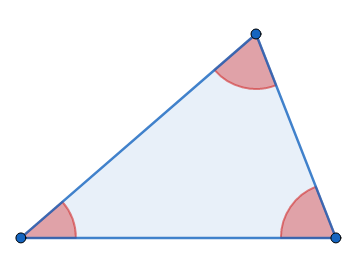
\includegraphics[width=2.5cm]{Image/Triangles/triangle_actuangle_complet.png}   \\

			\textit{Triangle}    & \textit{Triangle}       & \textit{Triangle} & \textit{Triangle}         & \textit{Triangle}           & \textit{Triangle}  \\
			\textit{équilatéral} & \textit{isocèle en $B$} & \textit{scalène}  & \textit{rectangle en $D$} & \textit{obtusangle en $G$}  & \textit{actuangle} \\
		\end{tabular}
	}
\end{center}


\newpage

\subsubsection{Mesure de l'aire d'un triangle}

Pour mesurer l'aire d'un triangle, nous allons chercher à le décomposer
en petits triangles rectangles, qui ont des aires plus simple à mesurer.

Dans un premier temps, commençons par voir comment l'on
calcul l'aire d'un triangle rectangle.

\paragraph*{Aire d'un triangle rectangle}

Prenons un triangle rectangle.
Dupliquons le, puis nous allons retourner
son jumeau afin de former un rectangle en assemblant les deux triangles.

L'aire d'un rectangle $\mathcal{A}_{\text{Rectangle}}$ est très facile à calculer,
c'est le produit de la Longueur ($L$) et de la largeur ($l$) du rectangle,
ainsi $\mathcal{A}_{\text{Rectangle}} = L \times l$.
Dans notre rectangle, qui est composé de deux triangles rectangles,
son aire est égal au produit des longueurs des deux cathètes.
On les nomme généralement $a$ et $b$, ainsi $2 \times \mathcal{A}_{\text{Triangle rectangle}} = a \times b$.

Nous nous intéressons à l'aire d'un seul triangle,
réarrangeons l'expression : $$ \mathcal{A}_{\text{Triangle rectangle}} = \frac{a \times b}{2} $$

\paragraph*{Aire d'un triangle quelconque}

Passons au cas général, l'astuce est de remarquer n'importe quel triangle
peut être découper en deux triangles rectangles,
et qui peuvent être dupliqués comme vu précédemment, pour former des rectangles.

Pour bien s'en rendre compte,
il peut être malin de pivoter le triangle,
en plaçant son côté le plus long à l'horizontal et orienté vers le bas.
Il est alors possible de tracer une droite verticale $d$ passant par le troisième sommet.
Cette droite sépare en deux triangles rectangles le triangle initial.
Il n'est pas obligatoire de suivre cette procédure,
mais cette dernière fonctionne toujours.

\medbreak

Et maintenant passons au calcul de l'aire,
pour le faire nous avons besoin de deux valeurs :

La longueur de la base (nommé $b$),
la base étant le côté du triangle étant perpendiculaire à $d$.
Cette base est la composition de deux cathètes, ayant comme longueur $b_1$ et $b_2$.
Ainsi, $b = b_1 + b_2$.

La hauteur (noté $h$),
qui est la distance entre le troisième sommet du triangle (celui ne faisant pas parti de la base) et le point d'intersection entre la droite et la base.

Ainsi, en combinant les deux triangles rectangles :
$$ \mathcal{A}_{\text{Triangle quelconque}} = \frac{b_1 \times h}{2} + \frac{b_2 \times h}{2} = \frac{(b_1+b_2) \times h}{2} = \frac{b \times h}{2} $$

\begin{center}
	\begin{tabular}{ccc}
		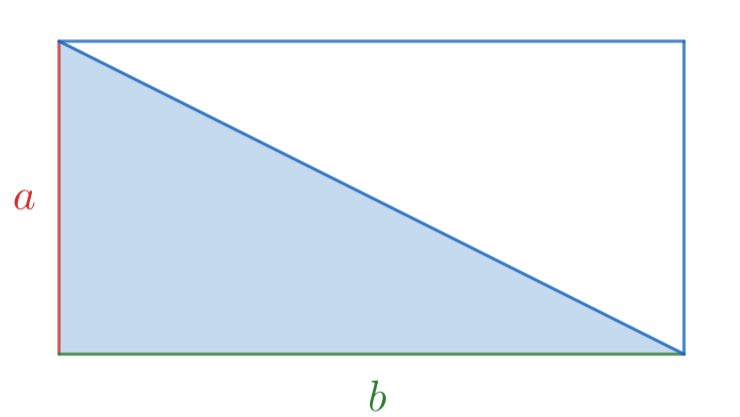
\includegraphics[width=6cm]{Image/Aire triangle rectangle.png} &               & 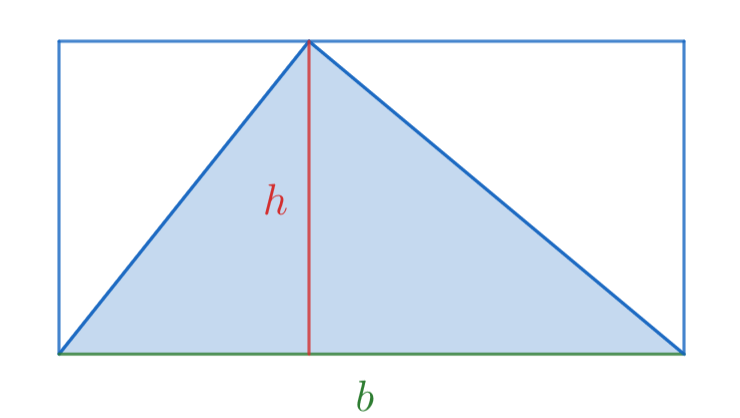
\includegraphics[width=6cm]{Image/Aire triangle quelconque.png} \\
		\textit{Aire d'un triangle rectangle}                          & \phantom{cou} & \textit{Aire d'un triangle quelconque}                          \\
	\end{tabular}
\end{center}

\paragraph*{Relation Aire-Périmètre}

\phantom{text}

Il est possible de majorer l'aire d'un triangle à l'aide de son périmètre, 
avec cette relation\footnote{
	Cette relation est démontrée en Annexe, à la page n°\pageref{relation_aire_perim_triangle}.
} :
$$ \mathcal{A}_{\text{Triangle}} \leq \frac{(p_{\text{Triangle}})^2 \sqrt {3}} {36} $$

\newpage

\subsubsection{Théorème de \textsc{Thalès}}

Prenons trois droites $(AB)$, $(BC)$ et $(CA)$.
Ces droites se croisent en formant un triangle.
Traçons une quatrième droite $(DE)$,

étant parallèle à l'une des droites précédentes,
disons par exemple que $(AB) // (DE)$.
On placera les points $D$ et $E$ sur les droites $(BC)$ et $(CA)$.

\begin{center}
	\begin{tabular}{ccc}
		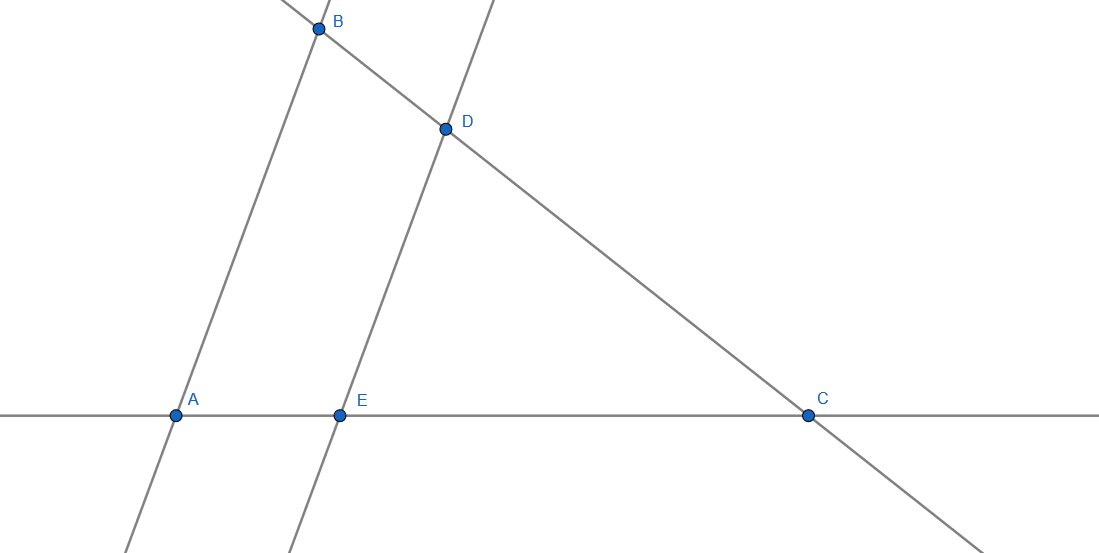
\includegraphics[width=6cm]{Image/triangle_tales_1.png} & 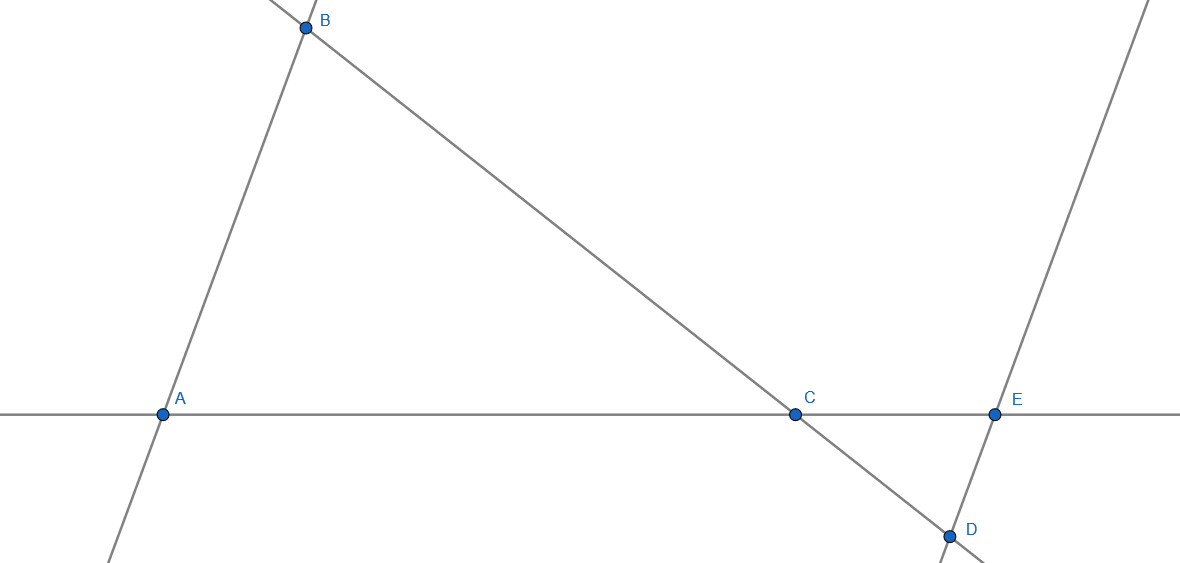
\includegraphics[width=6cm]{Image/triangle_tales_2.png} \\
		\textit{Cas de triangles imbriqués}                     & \textit{Cas de triangles opposés}                       \\
	\end{tabular}
\end{center}

Dans notre cas, les triangles $ACB$ et $ECD$ sont \emph{semblables},
c'est-à-dire qu'en agrandissant ou en réduisant le premier,
on peut retrouver le second. Ainsi deux triangles semblables
partagent les mêmes mesurent d'angles.

Le Théorème de \textsc{Thalès} traduit mathématiquement cette relation.
Il énonce que le facteur d'agrandissement ou de réduction est le même
pour tous les côtés.
Ainsi, on en déduit que : $$\frac{DE}{AB} = \frac{DC}{BC} = \frac{EC}{AC}$$

\paragraph*{Démonstration}

Cette démonstration se fonde sur le fait que l'aire
d'un triangle quelconque vaut,
peu importe la base choisi :

$$ \mathcal{A}_{\text{Triangle quelconque}} = \frac{b \times h}{2} $$

Les hauteurs des autres triangles $DEA$ et $DEB$ par rapport à
leur base commune $ED$ ont la même longueur,
du fait que $(AB)$ est parallèle à $(DE)$
(cette hauteur correspond à la distance la plus courte
entre les deux parallèles $(AB)$ et $(DE)$).

Comme ces deux triangles ont la même base et la même hauteur,
ils ont par conséquent la même aire.
Ils ont donc le même ratio (d'aires) avec n'importe quelle aire non nulle,
et en particulier celle du triangle $DEC$.

\medbreak

De plus, les hauteurs des triangles
$DEA$ par rapport à la base $[AE]$ et
celle de $DEC$ par rapport à la base $[EC]$,
sont confondues.

Ainsi, comme leur hauteur est la même,
le ratio des aires $DEA$ par $DEC$ est le même que
le ratio de leur bases $[AE]$ par $[EC]$.
Avec le même raisonnement, on en déduit que
le ratio des aires $DEB$ par $DEC$ est identique
au ratio des longueurs $BD$ par $DC$.

\medbreak

En réutilisant la première affirmation,
on en déduit que
le ratio de $AE$ par $EC$ est le même que
le ratio de $BD$ par $DC$.

\medbreak

On peut traduire ce raisonnement par les égalités suivantes :
$$\frac{AE}{EC} = \frac{{\text{Aire}}(DEA)}{{\text{Aire}}(DEC)}
	= \frac{{\text{Aire}}(DEB)}{{\text{Aire}}(DEC)}
	= \frac{BD}{DC}$$

\medbreak

\begin{center}
	\makebox[\textwidth][c]{
		\renewcommand{\arraystretch}{1.3}
		\begin{tabular}{rc|c}
			\multicolumn{2}{l|}{Prouvons maintenant que $\frac{EC}{AC} = \frac{DC}{BC}$ :} & \multicolumn{1}{l}{Prouvons que : $\frac{DE}{AB} = \frac{DC}{BC} = \frac{EC}{AC}$}                                             \\
			                                                                               &                                                                                    & Par construction des triangles,           \\
			Nous savons que :                                                              & $\frac{AE}{EC} = \frac{BD}{DC}$                                                    & les longueurs des côtés $AB$ et $DE$      \\
			Ainsi :                                                                        & $\frac{AE}{EC} + \frac{EC}{EC} = \frac{BD}{DC} + \frac{DC}{DC}$                    & dépendent directement des longueurs       \\
			C'est-à-dire :                                                                 & $\frac{AC}{EC} = \frac{BC}{DC}$                                                    & des deux autres côtés du triangle.        \\
			En inversant les fractions :                                                   & $\frac{EC}{AE} = \frac{DC}{BD}$                                                    & Ainsi le rapport entre ces deux longueurs \\
			                                                                               &                                                                                    & est bien égal aux autres rapports.        \\
		\end{tabular}
	}
\end{center}

\newpage

\subsubsection{Théorème de \textsc{Pythagore}}

Ce théorème énonce que dans un \textit{triangle rectangle},
la somme des longueurs mises aux carrées des cathètes (les côtés adjacents à l'angle droit),
est égal au carrée de la longueur de l'hypoténuse (le troisième côté du triangle).

Mathématiquement, on nomme classiquement les longueurs des cathètes $a$ et $b$ et celle
de l'hypoténuse $c$. En utilisant ces notations, on obtient :

\begin{center}
	$a^2 + b^2 = c^2$
\end{center}

Cette formule nous permet, si l'on connaît la longueur de deux côtés du triangle rectangle,
d'obtenir la longueur du troisième côté. Pour cela il faut remanier un peu le théorème de \textsc{Pythagore} :

\begin{center}
	\begin{tabular}{ccccc}
		$a = \sqrt{c^2 - b^2}$ &
		\phantom{text}         &
		$b = \sqrt{c^2 - a^2}$ &
		\phantom{text}         &
		$c = \sqrt{a^2 + b^2}$ \\
	\end{tabular}
\end{center}

\smallbreak

Ce théorème est l'un des plus élémentaires et incontournables du monde des mathématiques. 
Cette importance a poussé les mathématiciens à réaliser plus d'une centaine de démonstrations différentes, 
de ce théorème, voici mes deux préférées :

\paragraph*{Démonstration n°1 : Construction de carrés}

\textit{Conçue par Maurice Laisnez, en 1876.}

Prenons 4 copies d'un triangle rectangle (d'aire $\mathcal{A}_{\text{Triangle}}$), 
on notera sa plus petite cathète $a$, la plus grande $b$ et l'hypoténuse $c$.

Plaçons les de manière à former un carré avec les hypoténuses (comme sur la première illustration).
Dans ce premier cas, calculons $\mathcal{A}_{\text{Totale}}$, soit l'aire recouverte par toutes les figures.

Ainsi : $\mathcal{A}_{\text{Totale cas 1}} = 4 \times \mathcal{A}_{\text{Triangle}} + \mathcal{A}_{\text{Carré de côté }c}$

\medbreak

Déplaçons maintenant nos triangles afin de former deux plus petits carrés ayant respectivement 
comme longueur de côté $a$ et $b$. Ils ressemblent alors à la deuxième illustration. 

Dans ce cas : $\mathcal{A}_{\text{Totale cas 2}} = 4 \times \mathcal{A}_{\text{Triangle}} + \mathcal{A}_{\text{Carré de côté }a} + \mathcal{A}_{\text{Carré de côté }b}$

\medbreak

Dans les deux cas, l'aire totale est la même, 
car elle correspond toujours à l'aire d'un carré
de côté $a+b$.

\smallbreak

$\Longrightarrow \mathcal{A}_{\text{Totale cas 1}} = \mathcal{A}_{\text{Totale cas 2}}$

\smallbreak

$\Longrightarrow 4 \times \mathcal{A}_{\text{Triangle}} + \mathcal{A}_{\text{Carré de côté }c} = 4 \times \mathcal{A}_{\text{Triangle}} + \mathcal{A}_{\text{Carré de côté }a} + \mathcal{A}_{\text{Carré de côté }b}$

\smallbreak

$\Longrightarrow \mathcal{A}_{\text{Carré de côté }c} = \mathcal{A}_{\text{Carré de côté }a} + \mathcal{A}_{\text{Carré de côté }b}$

\smallbreak

$\Longrightarrow \mathbf{c^2 = a^2 + b^2}$


\begin{center}
	\begin{tabular}{cc}
		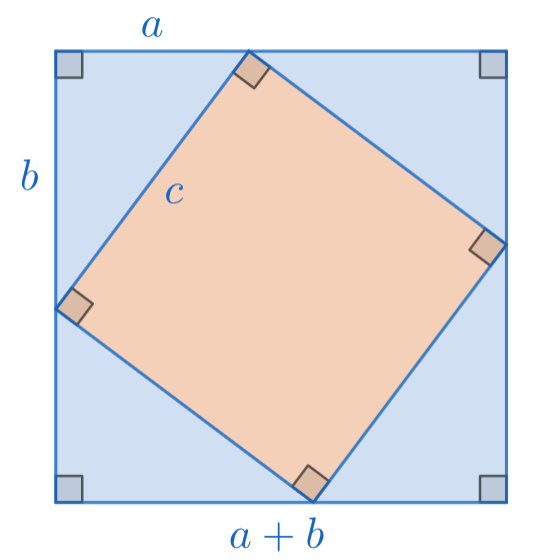
\includegraphics[width=6cm]{Image/Pythagore/laisnez_cas_1.png} & 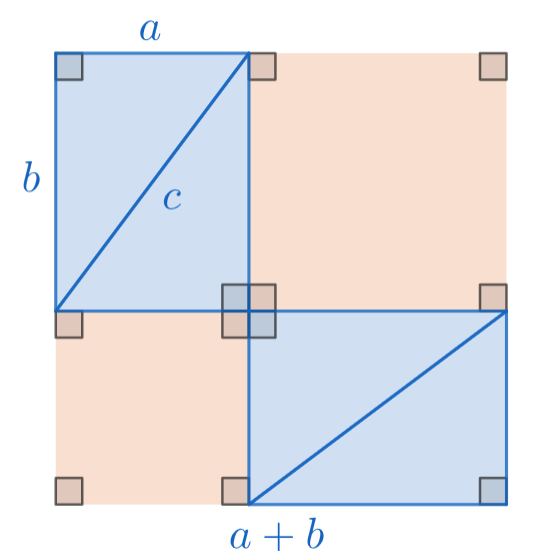
\includegraphics[width=6cm]{Image/Pythagore/laisnez_cas_2.png} \\
		\textit{Premier arrangement de triangles}                      & \textit{Second arrangement de triangles}                       \\
	\end{tabular}
\end{center}

\newpage

\paragraph*{Démonstration n°2 : Figure de l'hypoténuse}

\textit{Présentée dans le Zhoubi Suanjing}\footnote{
	Le \textit{Classique mathématique du Gnomon des Zhou}, ou \textit{Zhoubi Suanjing} 
	a été rédigé entre 1046 av. J.-C. et 220 (entre 8 954 et 10 220 E.H.),
	c'est un des plus anciens textes mathématiques chinois connus.
	C'est un recueil anonyme de problèmes mathématiques rencontrés 
	par le premier duc de la dynastie Zhou, \textsc{Ji Dan} et 
	son astronome et mathématicien \textsc{Shang Gao}.
	
	Ce recueil est le premier des \textit{Dix Canons du calcul}, 
	une collection d'ouvrages considérée comme texte 
	mathématique officiel pour les examens impériaux 
(examens ayant existé de 605 à 1905).}.

%https://fr.wikipedia.org/wiki/Zhoubi_Suanjing
%https://fr.wikipedia.org/wiki/Th%C3%A9or%C3%A8me_de_Pythagore#Par_le_puzzle_de_Gougu
%https://fr.wikipedia.org/wiki/Dix_Canons_du_calcul

Prenons 2 copies d'un triangle rectangle, 
on notera sa plus petite cathète $a$, la plus grande $b$ et l'hypoténuse $c$.

\smallbreak

Construisons un carré sur les hypoténuses de ces triangles, 
un carré (en jaune sur la première illustration), d'aire est $c^2$.

Découpons ce carré de manière à former deux autres copies des triangles initiaux,
en suivant le tracé indiqué sur la deuxième illustration.

\smallbreak

En déplaçant ces deux nouvelles copies,
il est possible d'obtenir deux carrés accolés, un de côté $a$, l'autre de côté $b$.
Ainsi, leurs aires sont respectivement égales à $a^2$ et $b^2$.

Et comme, lors d'un découpage, l'aire totale de toutes les pièces ne varie pas,
alors, l'aire du premier carré est égale à la somme des aires des deux plus petits carrés.

\smallbreak

Et donc : $c^2 = a^2 + b^2$

\begin{center}
	\makebox[\textwidth][c]{
		\begin{tabular}{ccc}
			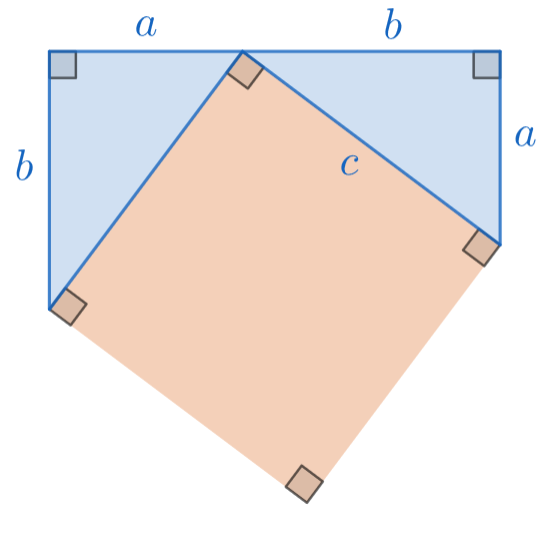
\includegraphics[width=5cm]{Image/Pythagore/figure_hypo_cas_1.png} & 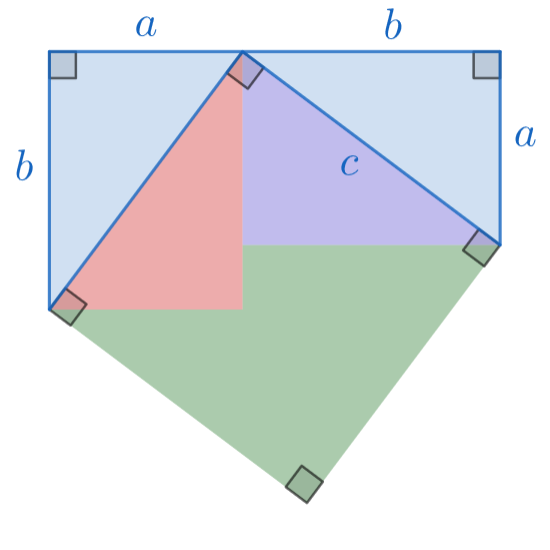
\includegraphics[width=5cm]{Image/Pythagore/figure_hypo_cas_2.png} & 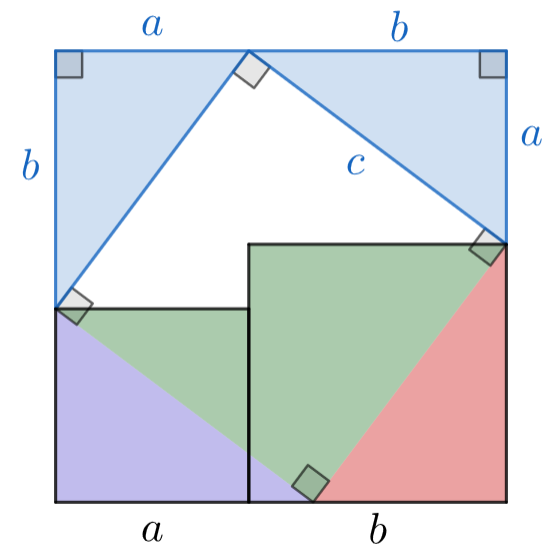
\includegraphics[width=5cm]{Image/Pythagore/figure_hypo_cas_3.png} \\
			\textit{Construction d'un}                                         & \textit{Découpage du carré}                                        & \textit{Formation de deux carrés}                                  \\
			\textit{carré de côté $c$}                                         & \textit{précédemment formé}                                        & \textit{de côtés $a$ et $b$}                                       \\
		\end{tabular}
	}
\end{center}

\subsubsection{Théorème d'\textsc{Al-Kashi}}

Le théorème d'\textsc{Al-Kashi} est une généralisation du théorème de \textsc{Pythagore}.

Il permet de calculer la longueur d'un côté d'un \textit{triangle quelconque},
si l'on connaît les longueurs des deux autres côtés et \textbf{l'angle former entre-eux}.
Malheureusement, ce théorème ne s'applique que dans le cas énoncé plus haut\footnote{
	Pour en savoir plus sur ce théorème et sur les autres formules utilisables dans les triangles,
	rendez-vous en Annexe, à la page n°\pageref*{al_kashi_autre_formule}. 
}.

Ce théorème utilise le \textit{cosinus},
une fonction trigonométrique, 
étant définie dans la Section 3, celle traitant de trigonométrie. 

\medbreak

Prenons un triangle quelconque, les longueurs de ses côtés sont $a$, $b$ et $c$ et 
les angles opposés à ces côtés sont respectivement $\alpha$, $\beta$ et $\gamma$ : 

\begin{center}
	\makebox[\textwidth][c]{
		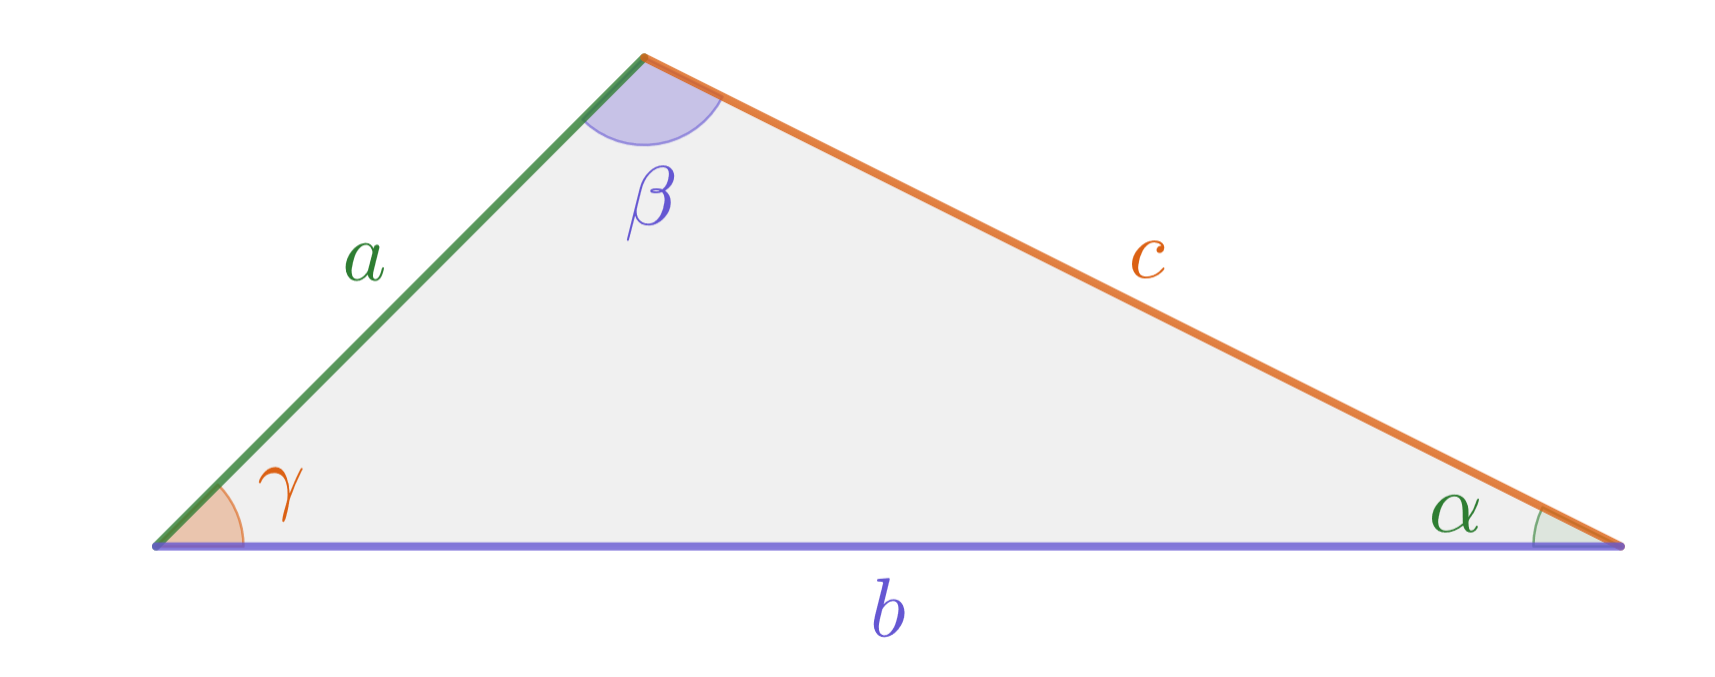
\includegraphics[width=6cm]{Image/Pythagore/Triangle Al-Kashi.png} 
	}
\end{center}

Grâce au théorème d'\textsc{Al-Kashi}, on peut établir les relations suivantes :

\begin{center}
	\begin{tabular}{ccccc}
		$a^2 = b^2 + c^2 - 2bc \cos(\alpha)$ &
		\phantom{text}                       &
		$b^2 = a^2 + c^2 - 2ac \cos(\beta)$  &
		\phantom{text}                       &
		$c^2 = a^2 + b^2 - 2ab \cos(\gamma)$ \\
	\end{tabular}
\end{center}



\newpage

\subsection{Les Quadrilatères} \label{quadrilateres}

Les quadrilatères sont des polygones à quatre côtés et la somme de leurs angles
intérieurs vaut $360^\circ$, $2 \pi$ rad ou $400$ gr.

\subsubsection{Classification des Quadrilatères}

La classification des Quadrilatères est plus complexes que celle
des Triangles, car la diversité des formes qu'ils peuvent prendre
est bien plus vaste que celle des Triangles.

\medbreak

On différencie deux familles de Quadrilatère :

\begin{itemize}
	\item[•] \textbf{Quadrilatère Croisé \textit{(ou complexe)}} : Quadrilatère ayant deux côtés se croisant.
	\item[•] \textbf{Quadrilatère Simple \textit{(ou non croisé)}} : Quadrilatère n'ayant aucun côtés qui se croise.
\end{itemize}

\bigbreak

La famille des \emph{Quadrilatères Simples} se décomposent en deux sous-familles :

\begin{itemize}
	\item[•] \textbf{Quadrilatère Concave} : Quadrilatère simple ayant au moins un angle intérieur rentrant.
	\item[•] \textbf{Quadrilatère Convexe} : Quadrilatère simple n'ayant que des angles intérieurs saillants.
\end{itemize}

\bigbreak

Parmi les \emph{Quadrilatères Convexes}, on trouve :

\begin{itemize}
	\item[•] \textbf{Quadrilatère (convexe) Inscriptible \textit{(ou Cyclique)}} : Quadrilatère convexe où l'on peut tracer un cercle passant par tous ses sommets.\footnote{
		      Un quadrilatère convexe est inscriptible
		      si et seulement si les quatre médiatrices des côtés
		      sont concourantes. Le point de concours est alors le centre
		      du cercle circonscrit et les médiatrices des diagonales
		      passent par ce point.}

	\item[•] \textbf{Trapèze (convexe)} : Quadrilatère convexe ayant deux côtés opposés parallèles entres eux. Ces côtés sont les \emph{bases} du Trapèze.
	\item[•] \textbf{Quadrilatère Circonscriptible \textit{(ou Tangentiel)}} : Quadrilatère dans lequel on peut tracer un cercle tangent à tout ses côtés.
	\item[•] \textbf{Quadrilatère Bicentrique} : Quadrilatère \textit{Inscriptible} et \textit{Circonscriptible}.
\end{itemize}

\bigbreak

Les \emph{Trapèzes} se décomposent eux-mêmes en différents types :

\begin{itemize}
	\item[•] \textbf{Trapèze isocèle} : Trapèze étant \textit{Inscriptible}. Il dispose de certaines propriétés\footnote{
		      Les deux bases du trapèze ont la même médiatrice, et celle-ci est un axe de symétrie du trapèze.
		      Ainsi, les deux angles adjacents à une même base sont égaux,
		      et les deux côtés n'étant pas les bases du trapèze ont la même longueur.
	      }.

	\item[•] \textbf{Trapèze circonscriptible} : Trapèze étant \textit{Circonscriptible}.
	\item[•] \textbf{Trapèze rectangle} : Trapèze possédant au moins un angle droit\footnote{Comme
		      les deux bases sont parallèles,
		      alors le trapèze rectangle possède au moins deux angles droits.}.
	\item[•] \textbf{Parallélogramme} : Trapèze \textit{Simple} dont les bases ont la même longueur,
	      ce qui implique que les deux autres côtés sont parallèles entre eux.
\end{itemize}

\bigbreak

On trouve parmi les \emph{Quadrilatères Circonscriptibles} :

\begin{itemize}
	\item[•] \textbf{Cerf-volant (convexe)} : Quadrilatère dont une des diagonales est un axe de symétrie.
\end{itemize}

\bigbreak

Et pour finir, certaines figures rentrent dans plusieurs groupes.

\begin{itemize}
	\item[•] \textbf{Losange (ou Rhombe)} : \textit{Cerf-volant convexe} dont tous les côtés ont la même longueur. C'est aussi un \textit{parallélogramme} où tous les côtés sont de la même longueur.
	\item[•] \textbf{Rectangle} : Quadrilatère étant un \textit{Parallélogramme}, un \textit{Trapèze isocèle} et un \textit{Trapèze rectangle}.
	      Ses côtés les plus longs sont appelés \emph{longueurs} (noté $L$) et les plus courts sont les \emph{largeurs} (noté $l$).
	\item[•] \textbf{Carré} : \textit{Losange} étant aussi un \textit{Rectangle}.
\end{itemize}

\newpage
\paragraph*{Diagramme de Venn récapitulatif}

\begin{center}
	\makebox[\textwidth][c]{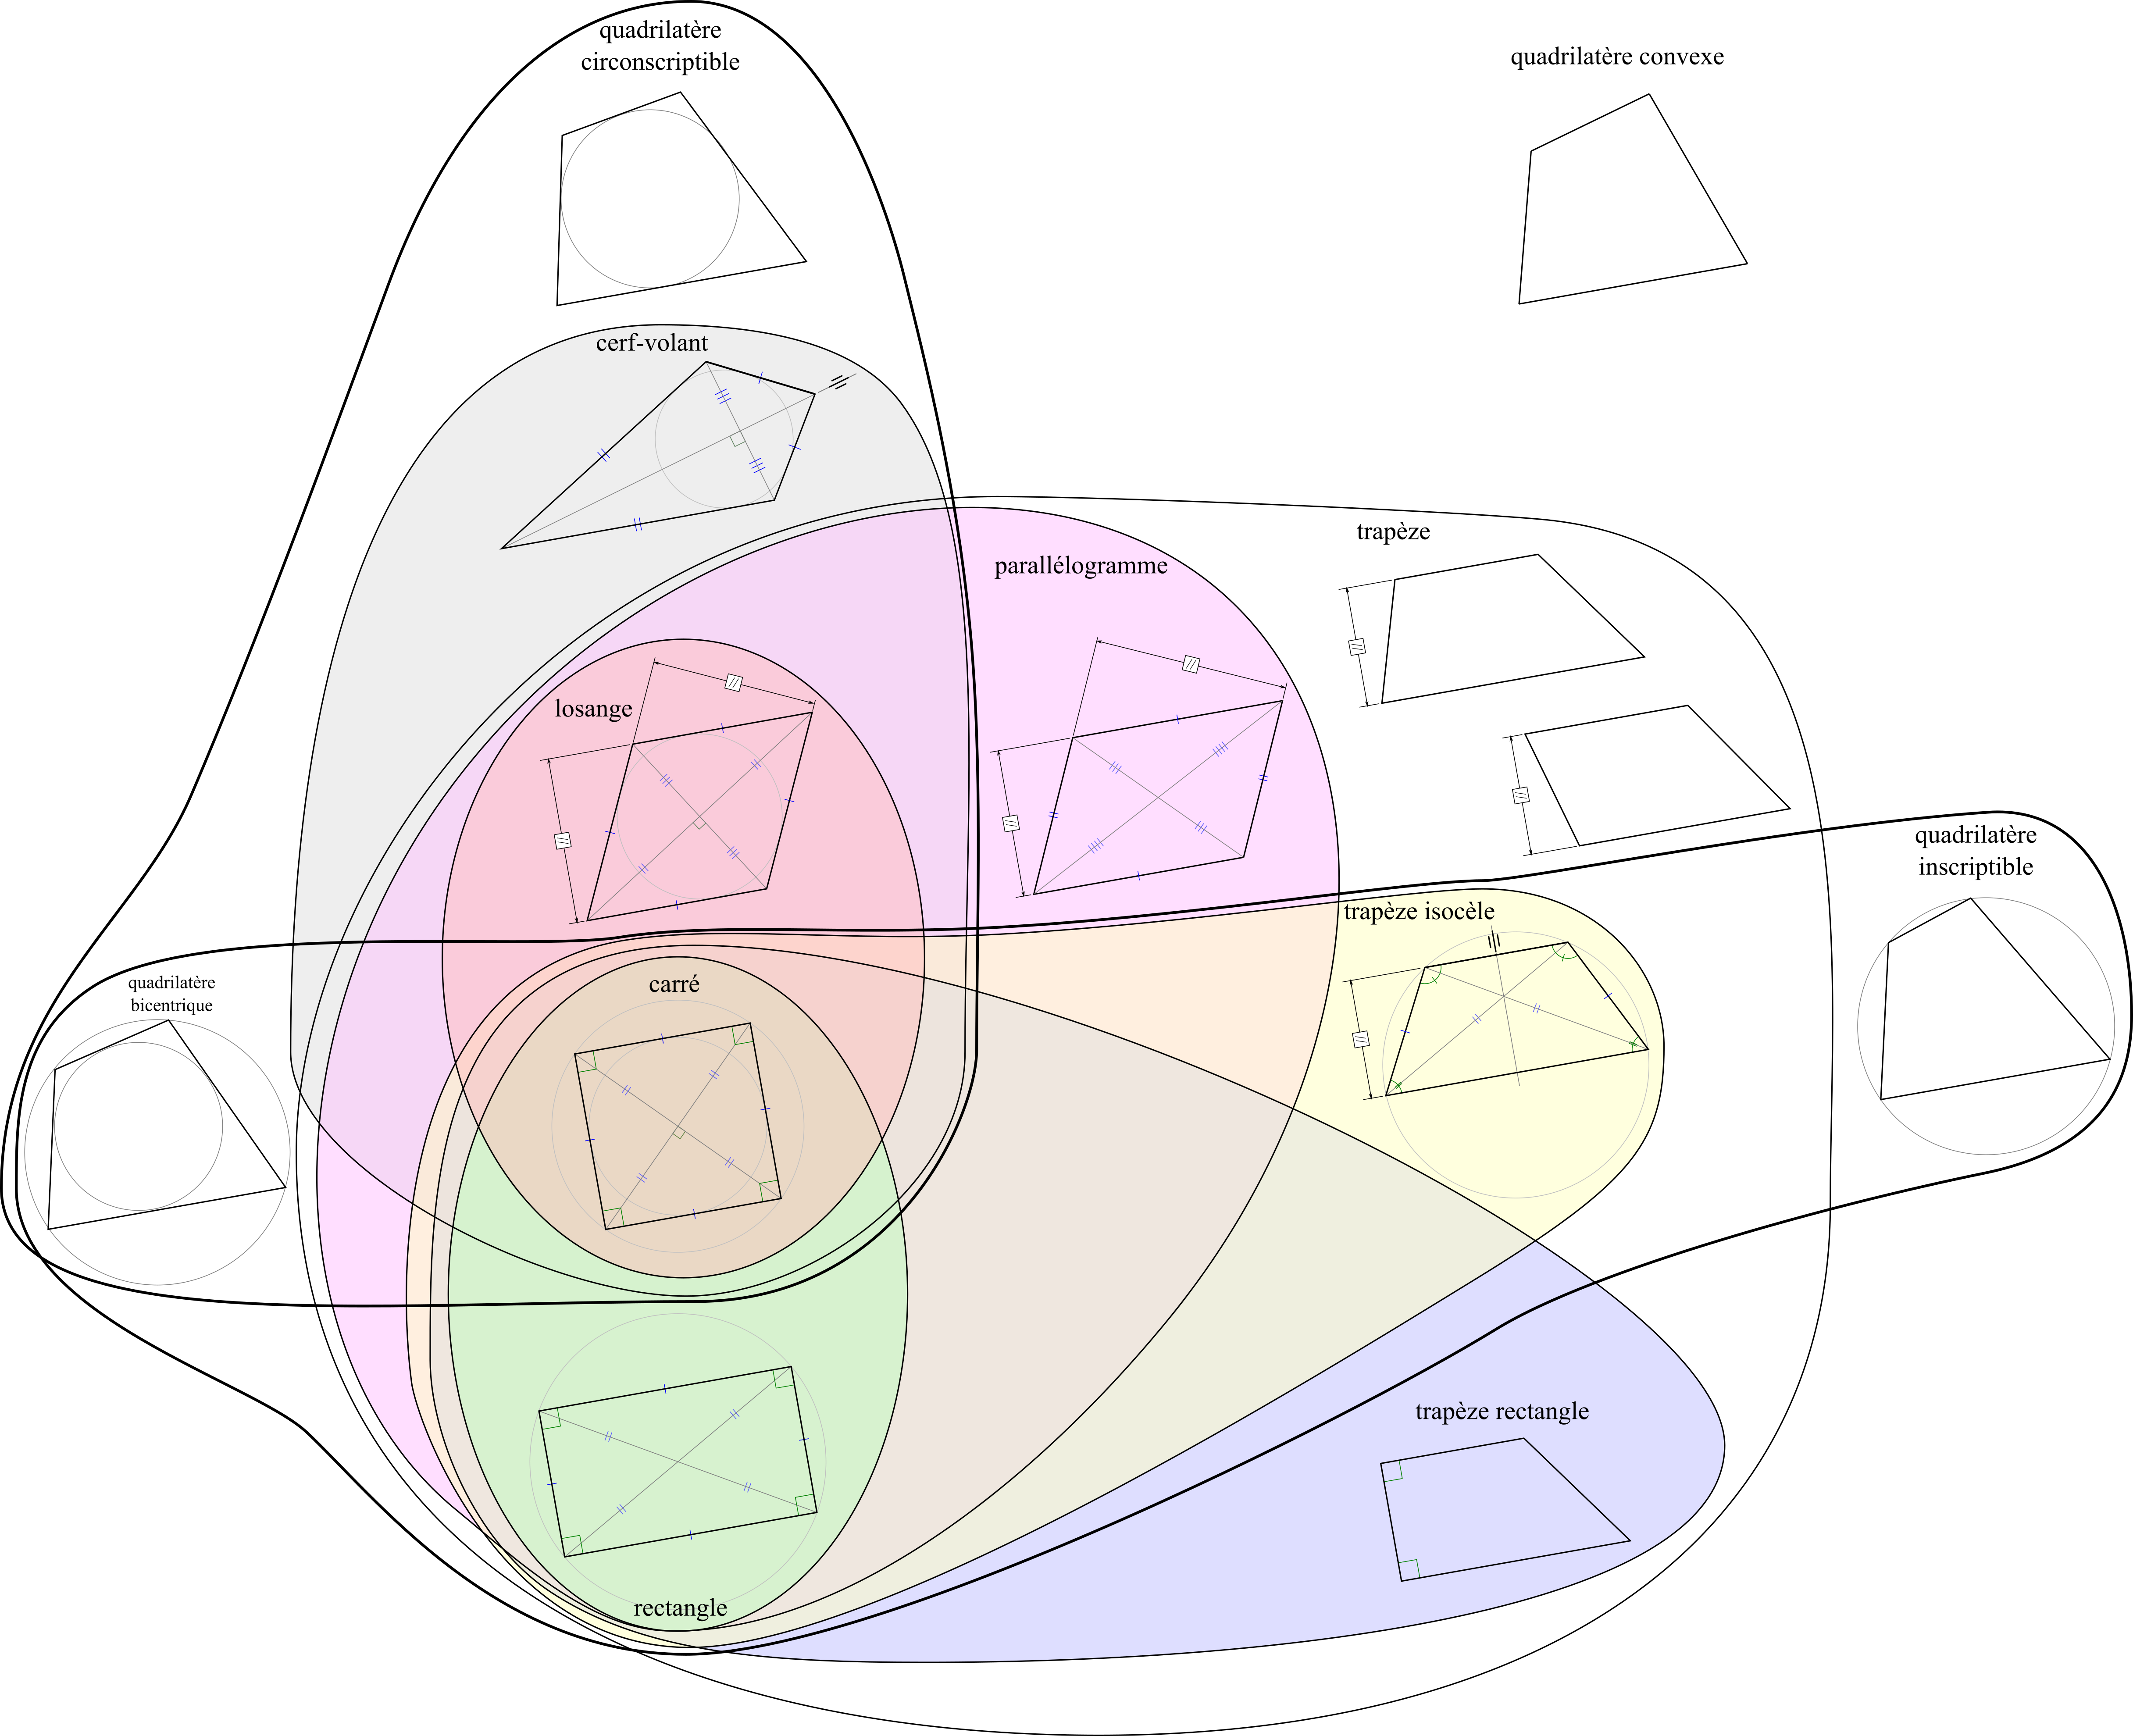
\includegraphics[width=16cm]{Image/Venn_type_quadrilateres.png}}
\end{center}

\vspace*{-0.5cm}

\subsubsection{Propriétés des Quadrilatères remarquables}

\paragraph*{Trapèze (convexe)}

Un quadrilatère convexe est un trapèze si et seulement si,
deux de ses côtés sont parallèles.
Cette propriété est équivalente au fait que,
ce quadrilatère possède une paire d'angles intérieurs
consécutifs de somme égale à un angle plat.
La somme des deux autres angles est alors la même.

\vspace*{-0.25cm}

\paragraph*{Parallélogramme}

Dans un parallélogramme, chaque côté est parallèle à celui lui étant opposé.
Cette propriété est équivalente à celle-ci : les diagonales du parallélogramme
se coupent en leur milieu. Le point d'intersection des diagonales est le centre de symétrie.
Les angles d'un parallélogramme qui se suivent sont supplémentaires.
Les angles opposés sont égaux.

Les \emph{bases} du parallélogramme sont ses côtés les plus longs.
La \emph{hauteur} du parallélogramme est la distance la plus courte entre ces deux bases.

\vspace*{-0.25cm}

\paragraph*{Losange}

Un losange est un quadrilatère équilatéral (tous les côtés ont la même longueur).
C'est aussi un parallélogramme ayant deux côtés consécutifs de même longueur.
Comme il était anciennement appelé \textit{rhombe},
ainsi l'adjectif qui lui est relatif est rhombique.

\vspace*{-0.25cm}

\paragraph*{Rectangle}

Un rectangle est un quadrilatère ayant 4 angles droits.
Vu autrement, c'est aussi un parallélogramme dont les diagonales ont la même longueur,
un quadrilatère équiangle (tous les angles sont égaux),
un parallélogramme inscriptible ou
c'est encore un parallélogramme ayant un angle droit.

\vspace*{-0.25cm}

\paragraph*{Carré}

Un carré est un quadrilatère équilatéral et équiangle, c'est ainsi un polygone régulier.
C'est un rectangle dont les diagonales sont perpendiculaires.
C'est à la fois un losange et un rectangle.

\subsubsection{Mesure de l'aire d'un Quadrilatère}

Il n'existe pas de formule de simple et fonctionnel pour obtenir l'aire
d'un quadrilatère quelconque. Cependant, il en existe pour certains quadrilatères :

\vspace*{-0.25cm}

\paragraph*{Quadrilatère convexe inscriptible \textit{(ou Cyclique)}}

L'aire d'un quadrilatère convexe inscriptible en fonction des longueurs a, b, c et d de ses
côtés successifs est donnée par la \emph{formule de Brahmagupta}\footnote{Plus d'information en Annexe, page n°\pageref*{formule_de_Brahmagupta}} :

$$ \mathcal{A}_{\text{Quadrilatère cyclique}} = \sqrt{(p_{\frac{1}{2}}-a)(p_{\frac{1}{2}}-b)(p_{\frac{1}{2}}-c)(p_{\frac{1}{2}}-d)} $$

où $p_{\frac{1}{2}} = \frac{a + b + c + d}{2}$ est le demi-périmètre.

\vspace*{-0.25cm}

\paragraph*{Cerf-volant (convexe)}

En dupliquant et en coupant le cerf-volant copié suivant les diagonales,
il est possible de construire un \textit{rectangle}.

Ainsi, l'aire d'un cerf-volant est égal au produit des longueurs
des diagonales ($d_{1}$ et $d_{2}$), divisé par deux.

$$\mathcal{A}_{\text{Cerf-volant}} = \frac{ d_{1} \times d_{2} }{ 2 }$$

\vspace*{-0.25cm}

\paragraph*{Trapèze (convexe)}

L'aire d'un trapèze (convexe) est égal à la somme des
deux bases ($B$ et $b$) multiplié par la hauteur ($h$) divisé par 2.\footnote{
	L'obtention de cette relation est légèrement plus complexe.
	On découpe le trapèze convexe en suivant une de ses diagonales,
	puis l'on va sommer les aires des deux triangles formés.

	Ainsi, $\mathcal{A}_{\text{Trapèze}} = \mathcal{A}_{\text{Premier triangle}} + \mathcal{A}_{\text{Second triangle}} = \frac{B \times h}{2} + \frac{b \times h}{2} = \frac {(B+b) \times h}{2}$
}

$$\mathcal{A}_{\text{Trapèze}} = \frac {(B+b) \times h}{2}$$

\vspace*{-0.25cm}

\paragraph*{Parallélogramme}

En découpant un parallélogramme,
il est possible d'obtenir un \textit{rectangle} de longueur égal à celle de ses bases ($b$),
et de largeur égal à sa hauteur ($h$).

$$\mathcal{A}_{\text{Parallélogramme}} = b \times h$$

\vspace*{-0.25cm}

\paragraph*{Losange}

Les losanges sont des cas particulier de \textit{cerf-volant},
ainsi, comme pour celui-ci :

$$\mathcal{A}_{\text{Losange}} = \frac{ d_{1} \times d_{2} }{ 2 }$$

\vspace*{-0.25cm}

\paragraph*{Rectangle}

L'aire d'un rectangle est égal au produit des longueurs de deux
côtés adjacents. Cette aire vaut donc le produit de la
longueur ($L$) et de la largeur ($l$) du rectangle.

$$\mathcal{A}_{\text{Rectangle}} = L \times l$$

\vspace*{-0.25cm}

\paragraph*{Carré}

L'aire d'un carré est égal au produit de la longueur d'un côté
($c$) par lui-même.\footnote{Lors que l'on calcul le produit d'un nombre
	par lui-même, on dit que l'on fait le “carré” de ce nombre.
	Ainsi, le carré de $5$ va être égal à $5 \times 5 = 5^{2} = 25$.}

$$\mathcal{A}_{\text{Carré}} = c^{2}$$

\newlength{\hauteurImage}
\setlength{\hauteurImage}{3.5cm}

\begin{center}
	\makebox[\textwidth][c]{
		\begin{tabular}{ccc}
			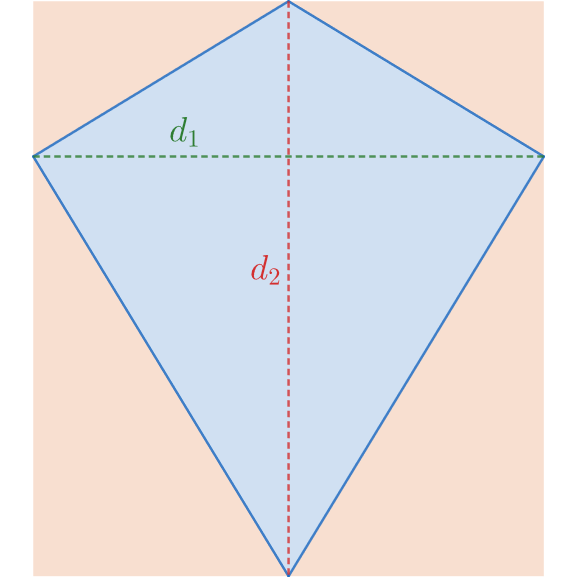
\includegraphics[height=\hauteurImage]{Image/Quadrilatère/aire_cerf_volant.png} & 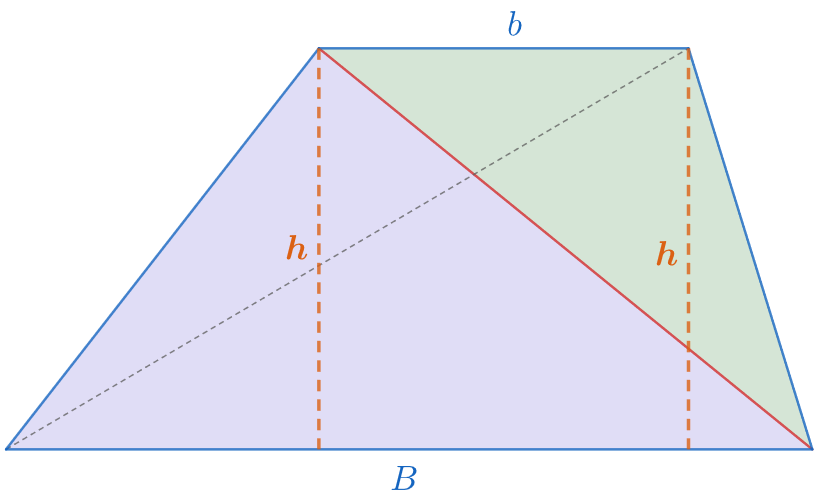
\includegraphics[height=\hauteurImage]{Image/Quadrilatère/aire_trapèze.png} & 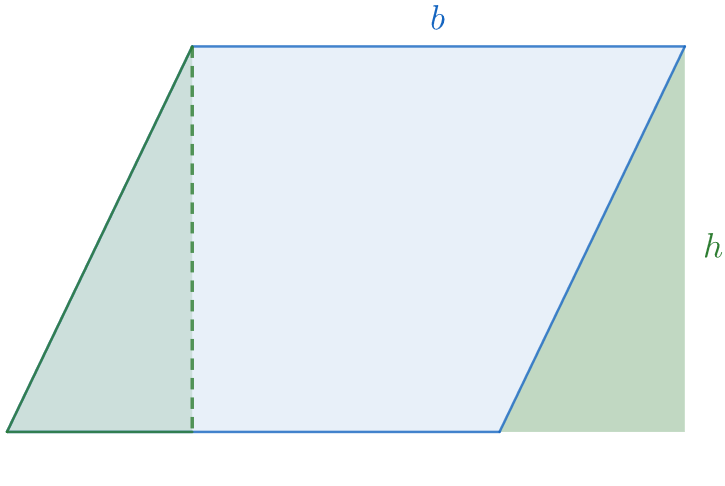
\includegraphics[height=\hauteurImage]{Image/Quadrilatère/aire_parallélogramme.png} \\
			\textit{Aire d'un cerf-volant}                                                  & \textit{Aire d'un trapèze}                                                  & \textit{Aire d'un parallélogramme}                                                  \\
		\end{tabular}
	}
\end{center}

\newpage

% -------------------------------------------------------------

\section{Les solides}

% -------------------------------------------------------------

\section{Annexe}

\subsection*{Géométrie non euclidienne} \label{geo_non_euclidienne}

\subsection*{Définition alternative de la mesure d'un angle} \label{autre_def_angle}

\subsection*{Définition du grade} \label{grade}

%[Grade (angle)](https://fr.wikipedia.org/wiki/Grade_(angle))

\subsection*{Différents symboles utilisés en Mathématique} \label{symboles_math}

%https://fr.wikipedia.org/wiki/Table_des_symboles_littéraux_en_mathématiques

\subsection*{Tracer une médiatrice ou une bissectrice} \label{tracer_mediatrice_bissectrice}

\subsubsection*{Tracer une Bissectrice}
Pointer le compas au sommet de l'angle et tracer un premier arc de cercle. Marquer les points d'intersection de cet arc avec les deux côtés de l'angle.

Pointer successivement le compas aux points d'intersection tracer deux arcs de cercle de même rayon (en gardant le même écartement du compas entre les deux opérations). Marquer le point d'intersection de ces deux arcs.

Relier le sommet de l'angle et le point d'intersection des deux derniers cercles et vous avez tracé la bissectrice de l'angle.


\subsection*{Démonstration de la formule de l'aire d'un cercle} \label{demo_formule_aire_cercle}


\subsection*{Histoire de $\pi$} \label{histoire_de_pi}

\subsection*{Approximations de $\pi$ et précision de celles-ci} \label{approximations_pi}

\subsection*{Nomenclature des polygone et des polyèdre} \label{nomenclature_polygone_polyèdre}

% https://fr.wikipedia.org/wiki/Pr%C3%A9fixe_num%C3%A9rique

\subsection*{Courbe de Jordan} \label{courbe_Jordan}

\subsection*{Polygones étoilés} \label{polygone_etoile}

\subsection*{Démonstration du lien entre la somme des angles et le nombre de côté d'un polygone} \label{demo_formule_lien_somme_angle_nb_cote}

cf cours n°1 et 2 - Brillant - Foundational Math
X = Somme angles ext = 360° (toujours)
Y = somme int + ext = 180°*n
somme int = Y - X


\subsection*{Démonstration des propriétés des axes de symétrie étant dans un polygone} \label{demo_axes_symétrie_polygone}

\textbf{Démonstration} : Si une droite est un axe de symétrie du polygone,
alors il faut déjà qu'il soit localement un axe de symétrie.
Prenons une portion d'un polygone, composé de deux segments $[AI]$ et $[IB]$.
Soit $d$ notre éventuel axe de symétrie, qui passe par le point $I$.

\smallbreak

\textit{1$^{\text{er}}$ cas - Seulement A et B sont des sommets du polygone}

Dans ce cas, $I \in [AB]$ et pour que $d$ soit un axe de symétrie,
il faut que $d\bot[AB]$, pour que le symétrique du segment $[AI]$ se
superpose parfaitement au segment $[IB]$.
De plus, les points $A$ et $B$ doivent se superposer,
on en déduit donc que,
$[AI]$ et $[IB]$ doivent mesurer la même longueur.
Ainsi, $d$ doit être perpendiculaire à $[AB]$ en passant par le milieu de ce segment.
C'est à dire, \emph{$d$ doit être la médiatrice de $[AB]$}.

\smallbreak

\textit{2$^{\text{ème}}$ cas - A, I et B sont des sommets du polygone}

Dans ce cas, de manière analogue au 1$^{\text{er}}$ cas,
pour que $d$ soit un axe de symétrie,
il faut que $d$ soit la bissectrice de $\widehat{BIA}$,
pour que le symétrique du segment $[AI]$ se
superpose parfaitement au segment $[IB]$.
De plus, les points $A$ et $B$ doivent se superposer,
on en déduit donc que,
$[AI]$ et $[IB]$ doivent mesurer la même longueur.
Ainsi, $d$ doit être la bissectrice de $\widehat{BIA}$ et $[AI]$ et $[IB]$ doivent mesurer la même longueur.
C'est à dire, \emph{$d$ doit être la bissectrice de $\widehat{BIA}$ en étant isocèle}.

On en conclue que, seul les médiatrices et les bissectrices isocèles peuvent être des
axes de symétrie d'un polygone.

\subsection*{Propriétés des triangles équilatérales} \label{propriete_triangle_equilateral}

Comme lors de la construction,
les deux cercles ont le même rayon,
la droite formée avec les deux points d'intersection est la médiatrice du segment initial.

Or, cette médiatrice est aussi un axe de symétrie du segment,
ainsi par symétrie, dans le triangle équilatéral terminé,
les angles ayant comme sommet les extrémités du segment initial font la même taille.

De plus, comme n'importe quel côté du triangle peut être choisi comme étant le "segment initial",
on trouve avec le même procédé 2 autres axes de symétrie,
ces derniers obligent tous les angles à être égaux par symétrie.

Et enfin, comme dans un triangle la somme des angles internes vaut $180^\circ$,
on en conclue que chaque angle vaut $\frac{180}{3} = 60^\circ = \frac{\pi}{3}$ rad.

\subsection*{Propriétés des triangles isocèles} \label{propriete_triangle_isocele}

\textbf{Démonstration} : La démonstration est analogue à la démonstration précédente :
Les deux points d'intersection des cercles forment la médiatrice du segment initial,
cette dernière est un axe de symétrie,
ce qui implique que les angles ayant comme sommet les extrémités du segment initial font la même taille.

\subsection*{Propriétés des triangles scalènes} \label{propriete_triangle_scalene}

\textbf{Démonstration} : Reprenons les démonstrations précédentes,
une médiatrice d'un des côtés du triangle est un axe de symétrie du triangle,
si et seulement si, le sommet du triangle n'étant pas une des extrémités du côté choisi,
se trouve sur cette médiatrice. Et pour que ce troisième point se retrouve sur la médiatrice,
il faut qu'il soit à la même distance des deux extrémités du côté,
et donc que deux côtés du triangle soit égaux.

De plus, si cette médiatrice passe par le troisième sommet,
alors elle aussi une bissectrice de l'angle ayant comme sommet ce troisième point.

Ainsi dans un triangle, les axes de symétrie sont des médiatrices et des bissectrices.
C'est à dire, pour rechercher des axes de symétrie, nous n'avons qu'à étudier les trois
médiatrices (ou les trois bissectrices) du triangle.

Dans un triangle scalène, comme tous les côtés mesurent des longueurs différentes,
alors aucune des médiatrices du triangle n'est un axe de symétrie,
car aucune des médiatrices ne passe par le "troisième sommet".

On en déduit que les triangles scalènes n'ont aucune axe de symétrie,
car dans les triangles, seules les médiatrices peuvent être des axes de symétrie.

Et donc, comme il n'y a aucun axes de symétrie dans ces triangles,
alors aucun de leurs angles ne mesurent la même valeur.

\subsection*{Démonstration de la relation Aire-Périmètre dans un Triangle} \label{relation_aire_perim_triangle}

\subsection*{Les Éléments d'Euclide} \label{euclide_element}

\subsection*{Autres formules utilisables dans les triangles} \label{al_kashi_autre_formule}

% Tableau résumant les cas d'utilisations des formules connues

\subsection*{Formule de Brahmagupta} \label{formule_de_Brahmagupta}

% https://fr.wikipedia.org/wiki/Quadrilat%C3%A8re_inscriptible#Aire


\newpage

\hfill

\textbf{BY} : L'œuvre peut être librement utilisée, à la condition de l'attribuer à l'auteur en citant son nom.

\textbf{NC} : Le titulaire de droits peut autoriser tous les types d’utilisation ou au contraire restreindre aux 
utilisations non commerciales (les utilisations commerciales restant soumises à son autorisation).

\textbf{SA} : Le titulaire a la possibilité d'autoriser à l'avance les modifications ; 
peut se superposer l'obligation pour les œuvres dites dérivées d'être proposées
au public avec les mêmes libertés que l'œuvre originales(sous les mêmes options Creative Commons).

\bigbreak

\makebox[14cm][r]{ 
\includegraphics[height=2cm]{Image/Licence/licence.png} }

\end{document}